%
% Master thesis template for Ghent University (2021)
%
%
%  !!!!!!!!!!!!!!!!!!!!!!!!!!!!!!!!!!!!!!!!!!!!!!!!!!!!!!!!!!!!
%  !!        MAKE SURE TO SET XeLaTex AS LATEX ENGINE        !!
%  !!!!!!!!!!!!!!!!!!!!!!!!!!!!!!!!!!!!!!!!!!!!!!!!!!!!!!!!!!!!
%  !! For overleaf:                                          !!
%  !!     1. click gear icon in top right                    !!
%  !!     2. select `XeLaTex` in "latex engine"              !!
%  !!     3. click "save project settings"                   !!
%  !!                                                        !!
%  !!!!!!!!!!!!!!!!!!!!!!!!!!!!!!!!!!!!!!!!!!!!!!!!!!!!!!!!!!!!
%
%
%  History
%    2014         Doctoral Thesis of Bruno Volckaert
%    2017         Adapted to master thesis by Jerico Moeyersons
%    2018         Cleanup by Merlijn Sebrechts
%    2021         Update by Marleen Denert and Merlijn Sebrechts with feedback from Leen Pollefliet
%    2022         Update by Merlijn Sebrechts
%
%  Latest version
%    https://github.com/galgalesh/masterproef-template
%

% Note: remove `openany` for printed version
\documentclass[11pt,a4paper,openany,english]{book}
\usepackage[a4paper,includeheadfoot,margin=2.50cm]{geometry}




\renewcommand{\baselinestretch}{1.2}  % stretch horizontal space between everything

\usepackage[hyphens]{url} % Break line on hyphens in long urls
\usepackage{graphicx}
\usepackage{tabularx}
\graphicspath{{images/}}
\usepackage{pdfpages}
\usepackage{enumitem}
\usepackage{float}
\usepackage{caption}
\usepackage{subcaption}
\captionsetup{justification=centering}
\usepackage[toc,page]{appendix}
\usepackage{fontspec}
\usepackage{pifont}
\newcommand{\cmark}{\ding{51}}
\newcommand{\xmark}{\ding{55}}

% Allow Japanese characters
\usepackage{xeCJK}
\setCJKmainfont{IPAMincho}
\setCJKsansfont{IPAGothic}
\setCJKmonofont{IPAGothic}

% Don't indent table of contents, list of figures, and list of tables
\usepackage{tocloft}
\setlength{\cftsecindent}{0pt}    % Remove indent for \section in Table of Contents
\setlength{\cftsubsecindent}{0pt} % Remove indent for \subsection in Table of Contents
\setlength{\cftfigindent}{0pt}    % remove indentation from figures in List of Figures
\setlength{\cfttabindent}{0pt}    % remove indentation from tables in List of Tables

\usepackage{parskip} % Add space between two paragraphs and don't indent the first line of the paragraph

\widowpenalty=10000
\clubpenalty=10000

% To generate fake lorem ipsum text
\usepackage{lipsum}



%
% UGent style guide
%
\setmainfont[
	Path=fonts/,
	BoldFont      =UGentPannoText-SemiBold.ttf,
	ItalicFont    =UGentPannoText-Normal.ttf,
	ItalicFeatures={FakeSlant=0.3},
	BoldItalicFont=UGentPannoText-SemiBold.ttf,
    BoldItalicFeatures={FakeSlant=0.3},
]{UGentPannoText-Normal.ttf}
\urlstyle{same} % Also use the default font for URLs


% If you want left justified text, uncomment the line below.
%\usepackage[document]{ragged2e} % Left justify all text

% Style Chapter titles so they have the chapter number in grey.
\usepackage{color}
\definecolor{chaptergrey}{rgb}{0.5,0.5,0.5}
\usepackage[explicit, pagestyles]{titlesec}
\titleformat{\chapter}[display]{\bfseries}{\color{chaptergrey}\fontfamily{pbk}\fontsize{80pt}{100pt}\selectfont\thechapter}{0pt}{\Huge #1}
\titlespacing*{\chapter}{0pt}{-80pt}{30pt}


% Header showing chapter number and title and footer showing page number
\newpagestyle{fancy}{%
  \sethead{} % left
          {} % center
          {\Large\thechapter~~\chaptertitle} %right
  \setfoot{} % left
          {\thepage} % center
          {} %right
  \setheadrule{0pt}
}
\pagestyle{fancy}

% Header showing chapter title and footer showing page number
\newpagestyle{numberless}{%
  \sethead{} % left
          {} % center
          {\Large\chaptertitle} %right
  \setfoot{} % left
          {\thepage} % center
          {} %right
  \setheadrule{0pt}
}

% We use the package `minted` for modern code highlighting.
\usepackage[newfloat,chapter]{minted}
\SetupFloatingEnvironment{listing}{name=Code Fragment, listname=List of Code Fragments}


\PassOptionsToPackage{hyphens}{url}
\usepackage{hyperref}
\usepackage{url}

\usepackage[authoryear]{natbib}
\bibliographystyle{apalike}
\usepackage[nottoc]{tocbibind}     % Put Bibliography in ToC

%
% Defines \checkmark to draw a checkmark
%
\usepackage{tikz}
\def\checkmark{\tikz\fill[scale=0.4](0,.35) -- (.25,0) -- (1,.7) -- (.25,.15) -- cycle;}

%
% For tables
%
\usepackage{booktabs}
\usepackage{array}
\usepackage{ragged2e}  % for '\RaggedRight' macro (allows hyphenation)
\newcolumntype{L}[1]{>{\raggedright\let\newline\\\arraybackslash\hspace{0pt}}m{#1}}
\newcolumntype{C}[1]{>{\centering\let\newline\\\arraybackslash\hspace{0pt}}m{#1}}
\newcolumntype{R}[1]{>{\raggedleft\let\newline\\\arraybackslash\hspace{0pt}}m{#1}}

\usepackage{polyglossia}
\setmainlanguage{english}

% Fix error "Package hyperref Warning: The anchor of a bookmark and its parent's must not be the same. Added a new anchor on ..."
\newcommand{\sectionbreak}{\phantomsection}

\usepackage[toc,acronym]{glossaries}  % for list of acronyms
\makeglossaries                       % start internal list of acronyms


%
% Set the title and your name
%
%%%%%%%%%%%%%%%%%%%%%%%%%%%%%%%%%%%%%%%%%%%%%%%%%%%%%%%%%%%%%%%%%%%%%%
%
% Add the specific info for your thesis
%
%%%%%%%%%%%%%%%%%%%%%%%%%%%%%%%%%%%%%%%%%%%%%%%%%%%%%%%%%%%%%%%%%%%%%%

\title{Discovering Digital Art Collections using Link-Traversal-based Query Processing}
\author{Martijn Bogaert}

%%%%%%%%%%%%%%%%%%%%%%%%%%%%%%%%%%%%%%%%%%%%%%%%%%%%%
% Add all the acronyms you use in your thesis here. %
% These will be added to the List of Acronyms       %
%%%%%%%%%%%%%%%%%%%%%%%%%%%%%%%%%%%%%%%%%%%%%%%%%%%%%

\newacronym{LD}{LD}{Linked Data}
\newacronym{LTQP}{LTQP}{Link-Traversal-based Query Processing}
\newacronym{IIIF}{IIIF}{International Image Interoperability Framework}
\newacronym{RDF}{RDF}{Resource Description Framework}
\newacronym{RDFS}{RDFS}{Resource Description Framework Schema}
\newacronym{OWL}{OWL}{Web Ontology Language}
\newacronym{JSON}{JSON}{JavaScript Object Notation}
\newacronym{JSON-LD}{JSON-LD}{JavaScript Object Notation for Linked Data}
\newacronym{HTML}{HTML}{HyperText Markup Language}
\newacronym{URI}{URI}{Uniform Resource Identifier}
\newacronym{HTTP}{HTTP}{Hypertext Transfer Protocol}
\newacronym{HTTPS}{HTTPS}{Hypertext Transfer Protocol Secure}
\newacronym{DNS}{DNS}{Domain Name System}
\newacronym{SPARQL}{SPARQL}{SPARQL Protocol and RDF Query Language}
\newacronym{FOAF}{FOAF}{Friend of a Friend}
\newacronym{CoGhent}{CoGhent}{Collections of Ghent}
\newacronym{N3}{N3}{Notation3}
\newacronym{XML}{XML}{Extensible Markup Language}
\newacronym{HMO}{HMO}{Human-Made Object}
\newacronym{DMG}{DMG}{Design Museum Gent}
\newacronym{HVA}{HVA}{Huis van Alijn}



%
%  END OF HEADER
%  The actual latex document content starts here.
%
\begin{document}
\frontmatter
\pagestyle{empty}

% Download the cover sheet from Plato
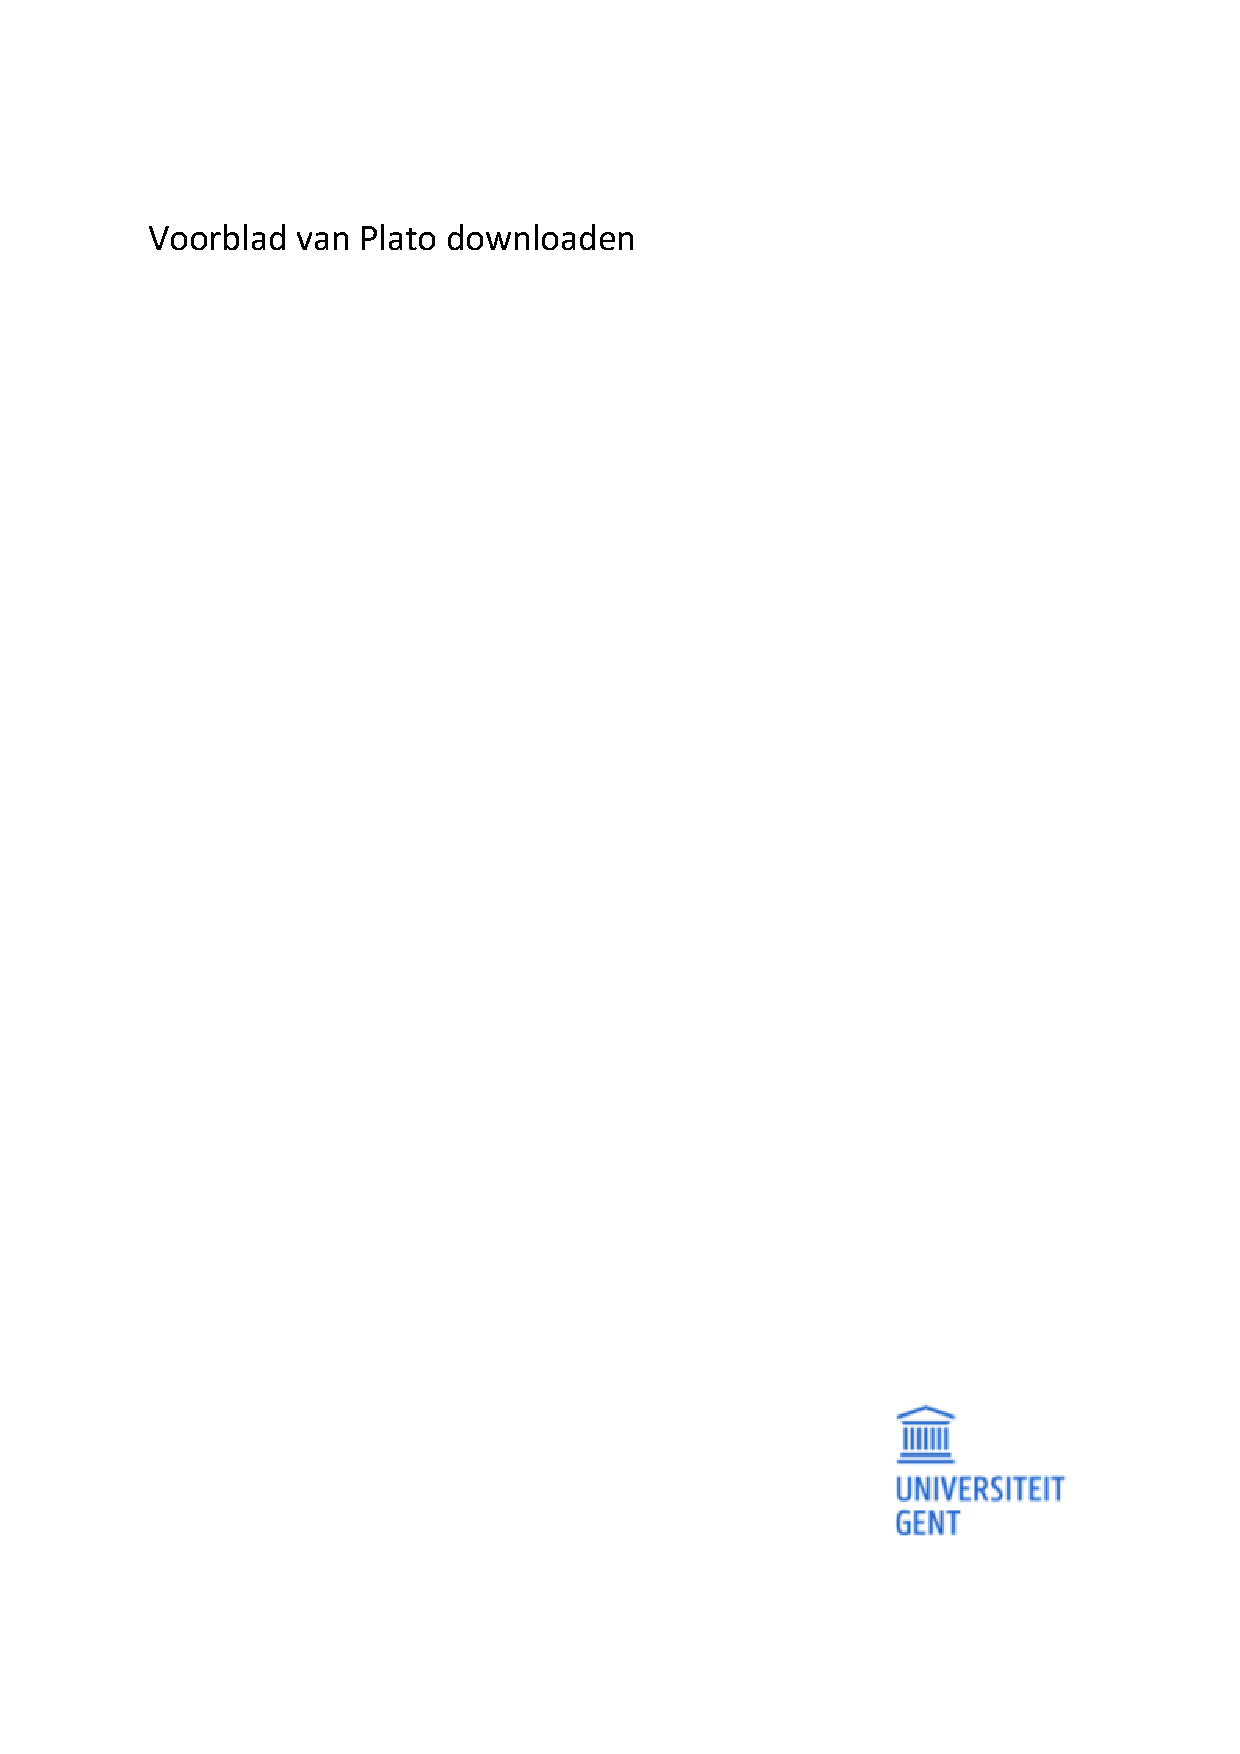
\includepdf{cover-sheet.pdf}

\pagestyle{plainpage}

\chapter*{Acknowledgements}

There are many people I would like to thank for their valuable advice and support over the past months. During those months, I have had the privilege of immersing myself in what has been an entirely new world for me, at the same time collaborating with very talented people. However, the past months have also been challenging. Therefore, a heartfelt thank you to those who have helped me navigate through them, is more than fitting.

First and foremost, I would like to express my sincere gratitude to Bryan-Elliott Tam. Bryan was my counselor throughout the second and third semesters of the academic year, going above and beyond to navigate me through the realm of link traversal. I distinctly recall one of our initial meetings. Bryan had prepared an entire PowerPoint presentation to help me get started with the new approach for my thesis, which we had decided on just the week before. I was able to dive right in. However, what I am most thankful to Bryan for, are his numerous reassuring and encouraging words during the more challenging moments. Especially during the last month, it brought me a great deal of comfort. So, Bryan, from the bottom of my heart: thank you.

Omdat ik met de volgende mensen in het dagelijkse leven steeds in mijn moedertaal communiceer, schakel ik even over naar het Nederlands. Dat doe ik in eerste instantie om Brecht Van de Vyvere te bedanken. Brecht was mijn begeleider tijdens het eerste semester van het academiejaar en heeft me mijn eerste stappen in de wereld van Linked Data helpen zetten. Dat deed hij altijd met veel zorg en de grootste glimlach. Dankjewel, Brecht.

Iemand die ik zeker niet mag en kan vergeten te bedanken, is Olivier Van D'huynslager. Als digitaal hoofd van CoGent heeft Olivier me bijna een volledig jaar lang mee begeleid. Op bijna elke meeting die ik met mijn begeleider hield, was Olivier aanwezig. Hij nam die extra vergaderingen er met de glimlach bij. Bedankt voor al je ideeën en goede raad, Olivier.

Ook Pieter Colpaert wil ik bedanken. Hij was anderhalf jaar geleden degene die me tijdens een wandeling in de Blaarmeersen kennis liet maken met de wereld van Linked Data. Dat deed hij met veel overgave en passie. Ik hoefde dan ook niet lang te twijfelen welk masterproefonderwerp ik zou kiezen. Bedankt, Pieter.

Dan zijn we aangekomen bij mijn familie. Ik ga het mezelf niet te moeilijk maken en meteen met mijn ouders beginnen. Zij zullen namelijk ook gemerkt hebben dat dit laatste jaar voor mij veruit de meest uitdagende van de voorbije zes was. Gelukkig heb ik de beste ouders die iemand zich kan wensen, en stonden zij trouw op de eerste rij om me er met aanmoedigende woorden en veel liefde doorheen te loodsen. Mama en papa, ik zal het jullie nog wel luidop zeggen, maar hier staat het alvast zwart op wit: dankjewel.

Wie ook zeker niet mag ontbreken op deze pagina, zijn mijn grootouders. Niet alleen tijdens het schrijven van mijn masterproef, maar jarenlang, tijdens elke examenperiode, mocht ik bij hen - gewoon het hoekje om - in alle rust komen werken. Elke dag opnieuw werd ik beladen met lekker eten, tussendoortjes, aanmoedigingen en vooral veel liefde. Ik heb veel onvergetelijke momenten meegemaakt tijdens mijn studententijd, maar ik lieg niet als ik zeg dat ik de dagen bij hen nog het meest zal missen. Lieve moemoe en grootva, ik ben jullie eeuwig dankbaar.

En dan is er nog iemand die ongetwijfeld niet kan wachten haar naam te horen. Mijn allerliefste Eva, dankjewel voor al die weken, maanden en jaren onophoudelijke steun. Ik weet niet hoe je het doet, maar zelfs op de moeilijkste momenten slaag je er telkens weer in mij op te rapen en met nieuwe moed vooruit te doen kijken. Ik kan niet wachten om met jou de volgende fase van mijn - ons - leven te beginnen. Ik zie je graag.

Ten slotte wil ik ook alle mensen die ik nog niet vermeld heb maar die me toch al die tijd gesteund hebben, heel oprecht bedanken. Ik denk daarbij aan familie, vrienden, medestudenten ... Die steun hoeft zelfs niet altijd uitgesproken te zijn. Een schouderklopje of een aanmoedigende glimlach kan al een wereld van verschil maken. Het zijn de kleine gebaren die het 'm doen. Dankjewel allemaal!
\chapter*{Toelichting in verband met het masterproefwerk}

Deze masterproef vormt een onderdeel van een examen. Eventuele opmerkingen die door de beoordelingscommissie tijdens de mondelinge uiteenzetting van de masterproef werden geformuleerd, werden niet verwerkt in deze tekst.

% This master's dissertation is part of an exam. Any comments formulated by the assessment committee during the oral presentation of the master's dissertation are not included in this text.

\subsection*{Melding van vertrouwelijkheid (enkel indien van toepassing)}

Bekijk hiervoor de informatie op \href{https://www.ugent.be/ea/nl/faculteit/studentenadministratie/masterproef/} {de facultaire website} - \textbf{Nota in verband met de vorm van de masterproef (alle opleidingen)}
\chapter*{Abstract}
\chaptermark{Abstract}
\addcontentsline{toc}{chapter}{Abstract}

\section*{English}

This master's thesis explores the innovative approach of discovering digital art collections using Link-Traversal-based Querying, focusing on the Collections of Ghent (CoGhent) data. CoGhent, a former partnership that digitized collections from cultural institutions, published the data as Linked Data in RDF format. By employing link traversal, this data can be explored in new ways, offering fresh insights into art collections.

The Comunica platform is central to this process, allowing for link traversal of RDF datasets and enabling the extraction of valuable data. In the CoGhent data, for instance, each entity referred to as a \textit{Human-Made Object}, such as an art piece, links to a IIIF Manifest. This manifest is a JSON-LD document that specifies artwork data and may provide instructions for digital display. Particularly, it holds a link to a picture of the piece, offering a visual representation of the artwork.

However, some resource links in the CoGhent data, notably Getty Vocabularies links, do not return an RDF compliant document, presenting a challenge for the Comunica link traversal engine. Workarounds are needed to reach the RDF compliant counterparts of these non-RDF compliant documents.

To make the discovery of CoGent collections accessible and assist art enthusiasts or professionals without a technical background in constructing SPARQL queries for a link traversal engine, two web application ideas are proposed. The first allows users to select predetermined properties of artworks, accompanied by a question indicating the purpose of the property. Each property corresponds to a sequence of predicates, which the application can ultimately use to generate a query. The second idea enables users to start from a resource of their choice, build a tree of predicates and objects, and eventually select objects of interest for query construction.

Ultimately, the discovered data can be incorporated in a IIIF Manifest, allowing display using a IIIF Viewer. This approach enhances the accessibility of art collections and provides a novel way to explore the rich cultural heritage in the CoGhent data.

\newpage
\newpagestyle{plainpage}{
  \sethead{}{}{}
  \setfoot{}{\thepage}{}
  \setheadrule{0pt}
}
\pagestyle{plainpage}

\section*{Nederlands}

Deze masterproef onderzoekt hoe digitale kunstcollecties met behulp van Link-Traversal-based Querying verkend kunnen worden. De focus ligt daarbij op de data die gepubliceerd werd door de Collectie van de Gentenaar (CoGent). Dit gewezen samenwerkingsverband digitaliseerde collecties van culturele instellingen en publiceerde de gegevens als Linked Data in RDF-formaat. Door link traversal te gebruiken, kunnen deze gegevens op nieuwe manieren worden verkend, wat leidt tot nieuwe inzichten in kunstcollecties.

Het Comunica-platform speelt een centrale rol in dit proces. Het maakt link traversal van RDF-datasets mogelijk, waardoor waardevolle gegevens kunnen worden verkregen. In de CoGent-data, bijvoorbeeld, verwijst elke entiteit die wordt aangeduid als een \textit{Mensgemaakt Object}, zoals een kunstwerk, naar een IIIF Manifest. Dit manifest is een JSON-LD-document dat kunstwerkgegevens specificeert en mogelijk instructies geeft voor digitale weergave. In het bijzonder bevat het een link naar een afbeelding van het stuk.

Echter, sommige resource-links in de CoGent-data, met name Getty Vocabularies-links, geven geen RDF-conform document terug. Hier kan Comunica niet mee aan de slag. Er zijn dus oplossingen nodig om de RDF-conforme tegenhangers te bereiken.

Om de ontdekking van CoGent-collecties toegankelijk te maken en kunstliefhebbers of professionals zonder technische achtergrond te helpen bij het opstellen van SPARQL-queries voor een link traversal engine, worden twee ideeën voor webapplicaties voorgesteld. Het eerste stelt gebruikers in staat om vooraf bepaalde eigenschappen van kunstwerken te selecteren, vergezeld van een vraag die het doel van de eigenschap aangeeft. Elke eigenschap komt overeen met een aaneenschakeling van predicaten, waarmee de applicatie uiteindelijk een query kan genereren. Het tweede idee stelt gebruikers in staat om vanuit een resource naar keuze, een boom van predicates en objecten op te bouwen, en finaal objecten van belang te selecteren voor queryconstructie.

Uiteindelijk kunnen de ontdekte gegevens worden toegewezen aan een IIIF Manifest, waarna een IIIF Viewer ze kan visualiseren. Deze benadering vergroot de toegankelijkheid van kunstcollecties en biedt een nieuwe manier om het rijke culturele erfgoed in de CoGent-data te verkennen.
% Write the extended abstract as a separate project using the IEEE conference proceedings template, and include the resulting PDF here in the document. You can find the template on Overleaf: https://www.overleaf.com/latex/templates/ieee-conference-template/grfzhhncsfqn. 

%Voeg dit toe als .pdf
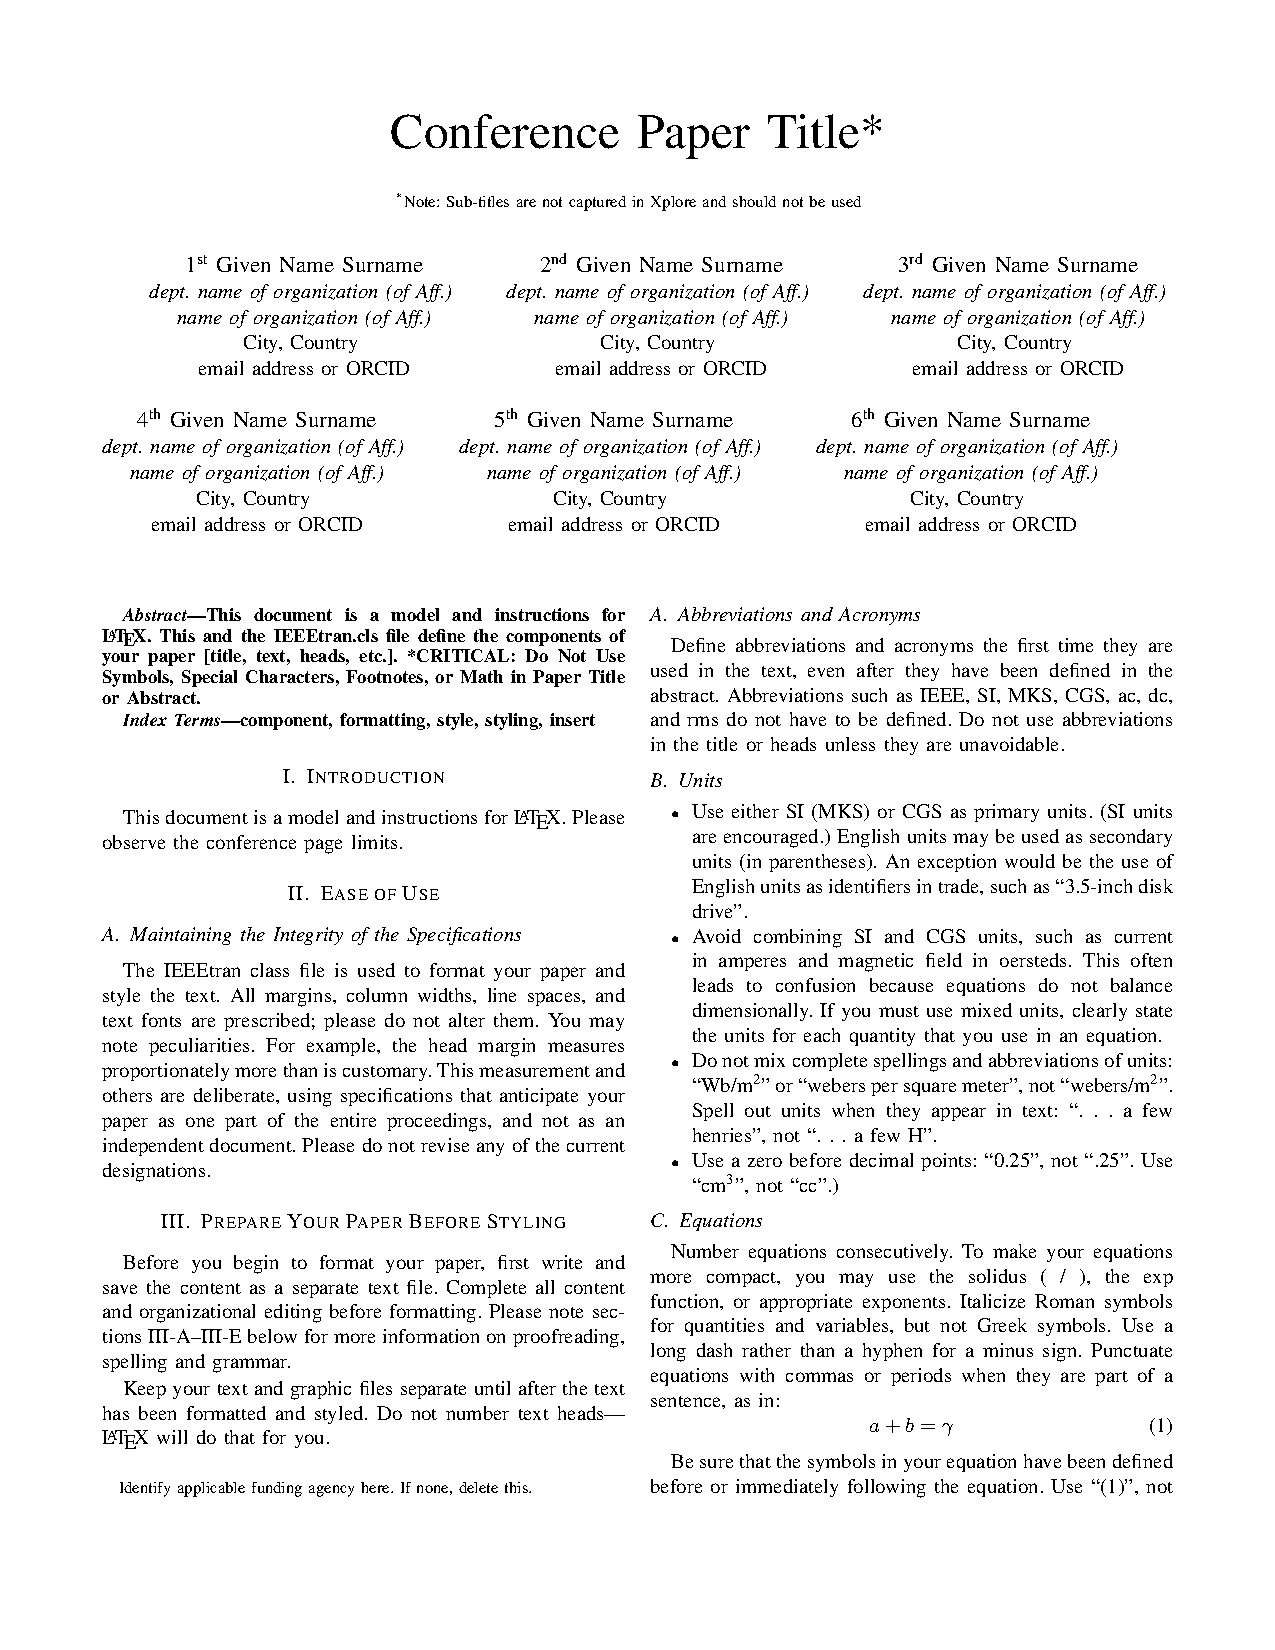
\includepdf[pages={-}]{abstract.pdf}  % Extended Abstract

\tableofcontents\newpage
\listoffigures\newpage
\listoftables\newpage
%%%%%%%%%%%%%%%%%%%%%%%%%%%%%%%%%%%%%%%%%%%%%%%%%%%%%%%%%%%%%%%
%                                                             %
% Note: To add or remove acronyms, modify `personal_data.tex` %
%                                                             %
%%%%%%%%%%%%%%%%%%%%%%%%%%%%%%%%%%%%%%%%%%%%%%%%%%%%%%%%%%%%%%%


% Print the glossary
\printglossary[type=\acronymtype, title={List of Acronyms}]

\glsaddallunused[\acronymtype]                              % make sure all unused acronyms are in list

\setlist[description]{style=standard} % reset list settings back to default

\listoflistings\newpage

%
% Include the main chapters of the thesis below
% Note: it's best to avoid spaces in filenames as Latex might complain about them.
%
\mainmatter
\pagestyle{fancy} % Use header
\chapter*{Introduction}
\chaptermark{Introduction}
\addcontentsline{toc}{chapter}{Introduction}

Digital art collections have long stood as a testament to human creativity and cultural evolution. With the advent of technology, many of these collections have undergone digitization, making them more accessible to a global audience. This digitization not only preserves the integrity of the artworks but also offers an opportunity for deeper exploration and understanding. However, with this digital transformation comes a set of challenges, especially for those without a technical background. Professionals in the cultural domain and general art enthusiasts, while passionate about art, may not possess the technical expertise to navigate and query these digitized datasets. This limitation can hinder their ability to make new discoveries and truly immerse themselves in the digital art world.

Discovering art collections can be interpreted in myriad ways. At its core, discovery is about unearthing new insights, understanding the nuances of each artwork, and drawing connections that might not be immediately apparent. This research primarily focuses on retrieving the inherent properties of cultural objects, delving into the intricate details that make each piece unique. However, the true potential of discovery lies in going beyond the confines of a single dataset. Link traversal offers this opportunity, allowing for a broader exploration that extends beyond the immediate dataset, unveiling new layers of knowledge and understanding.

By employing link traversal, one can uncover hidden relationships, gain a deeper understanding of cultural objects, and even compare different artworks in novel and enlightening ways. This approach is particularly beneficial when exploring the Collections of Ghent (CoGhent), a collaborative initiative between various cultural institutions. Published in a Linked Data format, the CoGhent collections are primed for link traversal, enabling a richer and more comprehensive exploration.

This research situates itself at the intersection of art and technology, aiming to bridge the gap between the two. It seeks to empower both professionals and art enthusiasts to navigate the digital art landscape, harnessing the power of link traversal to make new discoveries and draw meaningful connections. Through a systematic exploration of the Collections of Ghent and the development of tools tailored for query formulation, this research offers a roadmap for discovering digital art collections in their entirety.

Chapter~\ref{chap:rel_work} elucidates the foundational concepts of Linked Data and their real-world applications. It delves into the core principles, data modeling, and various RDF syntaxes, setting the stage for a deeper exploration of link traversal in the subsequent chapters. 

Chapter~\ref{chap:coghent_link_traversal} focuses on the CoGhent collections, highlighting the potential of link traversal for discovering properties of Human-Made Objects. It provides an overview of the available data sources and the development of a link traversal engine optimized for the objectives of this research.

In Chapter~\ref{chap:tools_query_building}, the emphasis shifts to the development of user-centric tools for query formulation. Two conceptual web applications are introduced, designed to alleviate the technical complexities of query formulation for users. The chapter also discusses the fundamental functionality shared by both web applications, ensuring a cohesive exploration throughout.

Lastly, Chapter~\ref{chap:handling_query_results} addresses the challenges of visualizing and preserving query results. It offers an overview of potential solutions, outlining their advantages and drawbacks, ensuring that the treasures within the CoGhent collections are accessible and meaningful to all.
\chapter{Related work}
\label{chap:rel_work}

\section{Linked Data}

This section presents a comprehensive exploration of Linked Data, encompassing its fundamental principles, data modeling, syntax, query interfaces, and the associated challenges and advantages. In Section~\ref{subsec:introduction_principles}, the concept of Linked Data and its principles are introduced, highlighting the significance of unique URIs, dereferencing, and data interlinking. Section~\ref{subsec:rdf} focuses on the Resource Description Framework (RDF) as the cornerstone for representing relationships and knowledge connections within Linked Data. Section~\ref{subsec:rdf_syntax} provides an overview of RDF syntax, including popular formats such as XML, Turtle, N-Triples, and JSON-LD, which facilitate the flexible expression and exchange of RDF data. Section~\ref{subsec:rdfs_owl} explores the Resource Description Framework Schema (RDFS) and Web Ontology Language (OWL), enabling the extension of Linked Data through ontology definition and enhanced semantic representation. Section~\ref{subsec:sparql} delves into SPARQL, the query language for Linked Data, and discusses various query interfaces that facilitate efficient data access and retrieval. Lastly, Section~\ref{subsec:challenges_advantages} examines the challenges and advantages of Linked Data, addressing aspects such as data quality, scalability, integration, and the benefits of improved interoperability and knowledge graph creation. This comprehensive examination provides a solid foundation for the subsequent discussions on linked traversal-based query processing.

\subsection{Introduction and Principles}
\label{subsec:introduction_principles}

To better understand the origins of the idea behind Linked Data, it is important to examine the origins of the World Wide Web. For example, its first, but still rather primitive, underlying technology was introduced in 1989 at CERN. Tim Berners-Lee was the man responsible for its development. By using HyperText Markup Language (HTML), it enabled scientists, and later the rest of the world, to publish documents that could contain links to other documents. This helped create a mesh of documents and information. However, since these documents in fact contained nothing more than raw data dumps and links between documents represented simply an indication of how to reach the document, these documents and their relationships lacked semantics. Figure~\ref{fig:no_linked_data} illustrates what a web of documents without unambiguous indications of what their contents and the links between them represent, might look like. It is necessary to note here that the used icons are not the contents of their respective documents, but only a representation of their contents. Nevertheless, in themselves, they prove the weakness of such web as much as when the effective content of the documents had been represented. After all, just from the raw content of documents and their mutual links, a person cannot clearly infer exactly what their constellation represents, let alone a computer. From that deficiency, therefore, emerged the idea of Linked Data. \citep{jacksi2019development} \citep{bizer2011linked}

\begin{figure}[htbp]
    \centering
	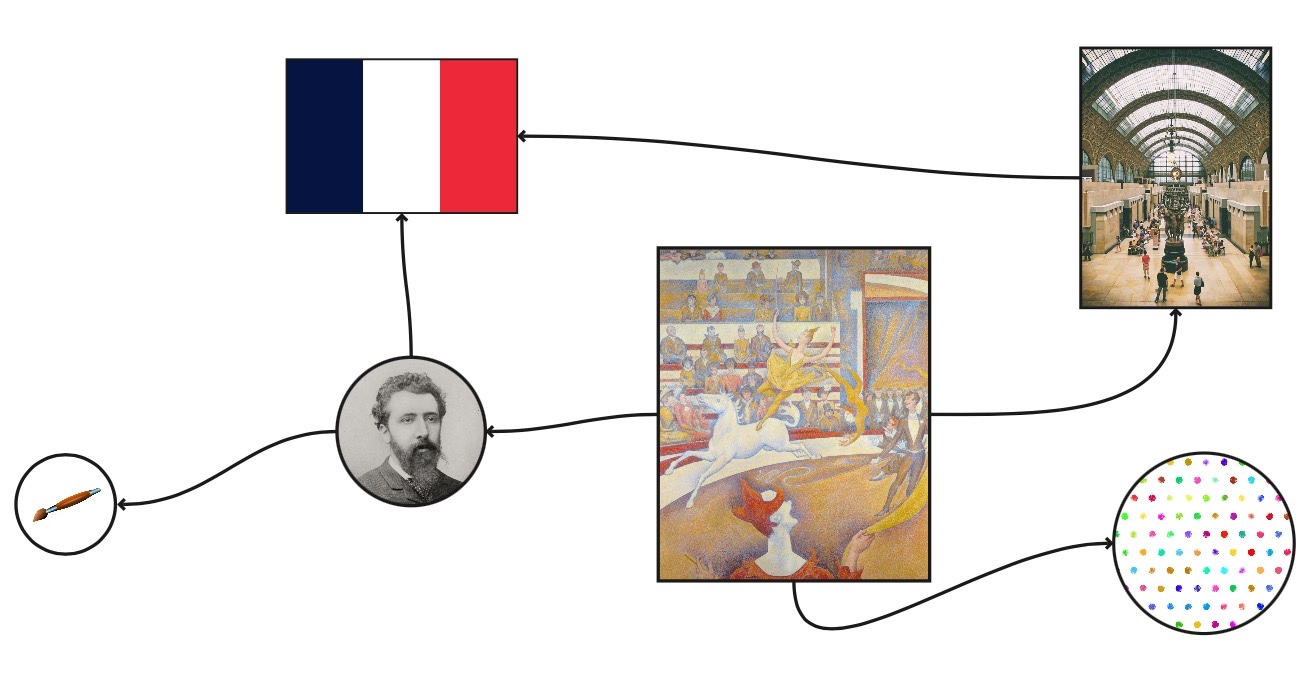
\includegraphics[width=\textwidth]{images/no_linked_data.jpg}
    \captionsetup{justification=centering}
	\caption{Representation of a web of documents without unambiguous indications of what the documents and the links between them represent}
	\label{fig:no_linked_data}
\end{figure}

Simply put, data coming from different sources can be labeled as Linked Data as soon as they are linked by typed links. In other words, links are no longer just an indication of how to reach another document. Indeed, within the Linked Data story, they also contain information about what exactly the link in question represents. Linked Data thereby ensures the meaning of data is explicitly defined, in turn rendering the data machine-readable. Figure~\ref{fig:linked_data} represents the same web of documents as Figure~\ref{fig:no_linked_data}, but this time in accordance with the idea of Linked Data. Indeed, the documents have been given an  unambiguous indication of what they represent, and their mutual semantics have also been clarified thanks to the labeling of their links. \citep{bizer2011linked}

\begin{figure}[htbp]
    \centering
	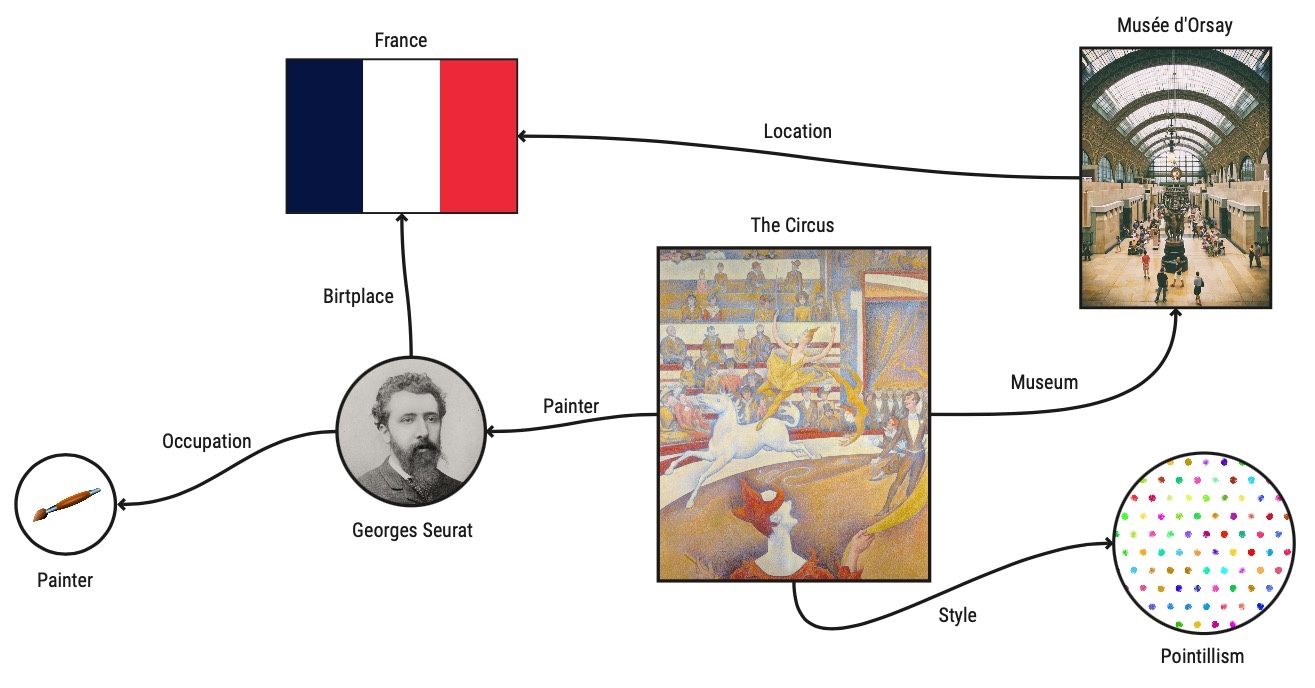
\includegraphics[width=\textwidth]{images/linked_data.jpg}
    \captionsetup{justification=centering}
	\caption{Representation of a web of documents composed according to the spirit of Linked Data}
	\label{fig:linked_data}
\end{figure}

Although several technologies exist to achieve the goals of Linked Data, the use of URIs is essential. After all, since URIs are unique, they can unambiguously reference a particular entity. Practically speaking, the URIs that appear in a Linked Data document can be dereferenced using the HTTP protocol in order to retrieve the underlying entities. For instance, \mintinline{text}{https://stad.gent/id/concept/530010539}, is a URI that can be dereferenced using the HTTP(S) protocol. By dereferencing URI after URI in this way, little by little a - what could be called - \textit{field of information} unfolds, whose semantics can be unambiguously determined by both man and machine. \citep{bizer2011linked}

To clarify the concept of Linked Data, \citet{berners2006linked} put forth four principles to be taken into consideration.
\begin{enumerate}

    \item \textbf{Use URIs as names for things}\\
    The principle of using URIs has already been discussed above.
    
    \item \textbf{Use HTTP URIs so that people can look up those names}\\
    The principle of using the HTTP protocol to dereference URIs was also touched on above. Nevertheless, it is important to reiterate its importance, as there are other protocols besides HTTP for dereferencing URIs. However, these will technically differ from the HTTP protocol, each in its own different ways. For example, not using the ubiquitous Domain Name System (DNS), is, among others, a common practice among alternative protocols. However, in light of clarity and uniformity, as well as for other technical reasons, the HTTP protocol should be adhered to. \citep{berners2006linked}
    
    \item \textbf{When someone looks up a URI, provide useful information, using the standards (RDF, SPARQL)}\\
    Obviously, it would not fit within the spirit of Linked Data to obtain a raw data dump when dereferencing a URI that was included from another document as a \textit{Linked Data link}. The obtained data itself must comply with Linked Data principles. Therefore, there are some standards that clearly indicate how ontologies can be described. Consequently, to enable the construction of applications that deal with Linked Data, it goes without saying that a Linked Data document should be built according to the principles of an existing standard. RDF, RDFS and OWL are common such standards and are therefore discussed further in Sections~\ref{subsec:rdf} and~\ref{subsec:rdfs_owl}. In addition, Section~\ref{subsec:sparql} introduces the SPARQL query interface. After all, large datasets are expected to also provide such interface. \citep{berners2006linked}
    
    \item \textbf{Include links to other URIs so that they can discover more things}\\
    The fourth and final principle, too, is rather obvious. After all, by definition, one can only speak of Linked Data when a document refers to at least one other document. In addition, to help advance the cause of transforming the World Wide Web in its current form into a semantic World Wide Web, aided by the concepts of Linked Data, it is preferable to also include links to documents belonging to other sites. \citep{berners2006linked}
    
\end{enumerate}

In conclusion, Linked Data plays a crucial role in giving meaning to the Web by enabling the interconnection and integration of diverse data sources. By adhering to the principles of unique URIs, dereferencing, linking, and using standardized formats, Linked Data fosters a more structured and interconnected web of knowledge. Examples such as DBpedia\footnote{\href{https://www.dbpedia.org}{https://www.dbpedia.org}}, which provides a structured representation of Wikipedia data, and Friend of a Friend (FOAF), which allows for the description of people and their relationships, illustrate how publishing data as Linked Data benefits from enhanced data discoverability, interlinking with other datasets, and enabling novel applications and insights. Local initiatives like Collections of Ghent (CoGhent\footnote{\href{https://www.collections.gent}{https://www.collections.gent}}), which digitizes art collections from cultural houses in Ghent and will be further discussed in Section~\ref{sec:coghent}, similarly demonstrate the potential of Linked Data for local organizations in contributing to the broader web of knowledge. \citep{auer2007dbpedia} \citep{golbeck2008linking} \citep{van2022publishing}

\subsection{Resource Description Framework}
\label{subsec:rdf}

The idea behind Linked Data is interesting in itself, but does not yet describe exactly how to get started with it. Therefore, this section introduces the Recourse Description Framework (RDF). Developed under the auspices of the World Wide Web Consortium (W3C), RDF is an infrastructure that allows for the construction of Linked Data datasets and their metadata. Consequently, this not only allows data publishers to lay out their data as Linked Data, but also gives data consumers clear guidance on how the data can be understood. Note here that data consumers can be both individuals and computer applications. \citep{miller1998introduction}

An interesting way to understand RDF is to first make a jump to the English language. Take the sentence below:
\begin{center}
    \textbf{The birthplace of Georges Seurat is France.}
\end{center}
According to English grammar, the \textit{who} or \textit{what} around which a sentence revolves, is called the subject of the sentence. Therefore, when looking at the sentence above, \textit{Georges Seurat} is its subject. In addition, the part of a sentence that gives more information about the subject, is referred to as the predicate, making \textit{the birthplace} the predicate in the above sentence. Finally, the matching value complementing the predicate and completing the sentence, is also of importance. Logically, in the case of the sentence above, that would be \textit{France}. Together, these three components form the most basic building blocks of a sentence. In fact, no matter their lengths, combined, they will always establish a piece of knowledge, exactly what RDF also seeks to accomplish. \citep{powers2003practical}

The building blocks of RDF data are basically exactly the same as those of linguistic sentences. After all, they are also three in number and even partly share the same names. Moreover, much like with sentences, combined, they form a single yet very clear piece of knowledge. Unlike the English language, however, they are not referred to as sentences. Rather, they are called triples. \citep{powers2003practical}
\begin{itemize}

    \item \textbf{Resource}\\
    \cite{miller1998introduction} defines a resource as any object that is uniquely identifiable by a URI. This enables it to come in different forms: as a web page, as an entire website or simply as any resource on the Web that conveys information in one way or another. \citep{candan2001resource}
    
    To make the comparison with the English language again, in a triple, the resource corresponds to the subject in a sentence. Moreover, in practice, the term \textit{subject} is often preferred over \textit{resource}. \citep{powers2003practical}

    \item \textbf{Property Type}\\
    A property type, or simply a property, introduces a specific aspect, characteristic, attribute, or relationship of a resource. A property type always expects a value to ultimately define the piece of knowledge represented by a triple. \citep{candan2001resource} \citep{miller1998introduction}
    
    As for property types, in practice, the corresponding term from the English language, \textit{predicate}, is also frequently used as opposed to the more theoretical \textit{property type}. \citep{powers2003practical}

    \item \textbf{Value}\\
    A value resolves the concept or relationship initiated by a property type. In this way, it captures the knowledge conveyed by the triple. Values can be represented as text strings, numbers, or any atomic data. However, they can also be resources themselves. This characteristic allows triples therefore to be the building blocks of a web of knowledge. \citep{miller1998introduction}
    
    It is evident that a value in a triple corresponds to a value in an English sentence. However, in practice, the term \textit{object} is often preferred. \citep{powers2003practical}
    
\end{itemize}

While triples convey a clear and distinct piece of knowledge, a collection of triples can naturally convey a more comprehensive knowledge. Such a collection of triples, interconnected by values that are themselves resources, is also referred to as an \textit{RDF description}. Figure~\ref{fig:rdf_description} illustrates what such an RDF description might look like. Additionally, it is important to note that each of its components, whether it be a resource, property type, or value, does not necessarily have to be a digital concept. After all, Web assets can perfectly represent real-life concepts. \citep{miller1998introduction} \citep{candan2001resource}

\begin{figure}[htbp]
    \centering
	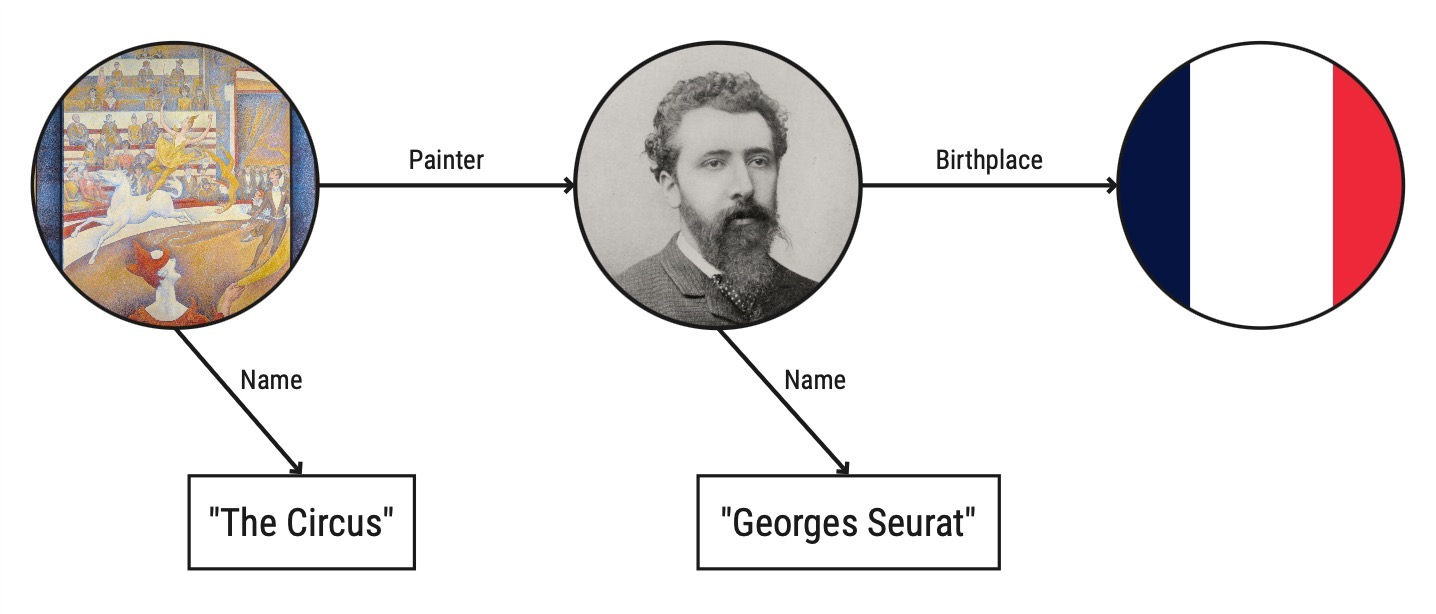
\includegraphics[width=\textwidth]{images/rdf_description.jpg}
    \captionsetup{justification=centering}
	\caption{Representation of an RDF description}
    \caption*{Circles represent resources, arrows represent property types and values are situated at the end of arrows}
	\label{fig:rdf_description}
\end{figure}

Clearly, different terms exist to denote the same RDF concepts. For instance, in addition to the synonyms mentioned above, in literature, the term \textit{statement} is sometimes preferred over \textit{triple}. However, in light of uniformity and clarity, throughout the rest of this text, the terms \textit{triple}, \textit{subject}, \textit{predicate} and \textit{object} will be used instead of their counterparts. \citep{candan2001resource}

\subsection{Resource Description Framework Syntax}
\label{subsec:rdf_syntax}

What constitutes RDF exactly, should be clear by now, but the question of how to actually write down RDF descriptions, still remains to be answered. Therefore, this section introduces some RDF syntaxes. However, since they are not the focus of this research, they will not be discussed in detail. Instead, their outlines will be illustrated by presenting the RDF description from Figure~\ref{fig:rdf_description} in the syntax in question. Incidentally, since the schema presented in Figure~\ref{fig:rdf_description} also has clear guidelines on how to be used, in itself, it also qualifies as an RDF syntax, albeit a graphical one. \citep{miller1998introduction}

All the syntaxes to be discussed are instantiations of the RDF Model and Syntax Specification, providing concrete implementations. However, the first syntax stands apart from the rest as it primarily serves as a notation recommendation for humans to express RDF descriptions in a manner that is unambiguous yet simple. Unlike the other syntaxes, this particular one is not intended for machine consumption. Code Fragment~\ref{lst:human_rdf_syntax} demonstrates how the RDF descriptor, as schematically depicted in Figure~\ref{fig:rdf_description}, can be represented using this human-centric syntax. In this representation, resources are enclosed in straight brackets, while property types are represented by arrows. Furthermore, the representation of values varies depending on their types. As denoted, resources are encapsulated within brackets. However, if the values are atomic in nature, they are simply enclosed in quotation marks. \citep{miller1998introduction}

\begin{listing}[htbp]
    \begin{minted}[samepage]{text}
[The Circus] ------name--------> "The Circus"
[The Circus] ------painter-----> [Georges Seurat]
[Georges Seurat] --name--------> "Georges Seurat"
[Georges Seurat] --birthplace--> [France]
    \end{minted}
    \caption{RDF description depicted using a human-centric RDF syntax}
    \label{lst:human_rdf_syntax}
\end{listing}

The example from Code Fragment~\ref{lst:human_rdf_syntax} is easy to read, but at the same time rather confusing. Indeed, certain resource names correspond to certain atomic values. One could of course try to give the resources a more generic name to indicate what exactly the resource in question means. However, that would make little sense given the way the following machine-readable RDF syntaxes refer to resources. After all, they use URIs, allowing for a more clear distinction between resources and atomic values.

\begin{itemize}

    \item \textbf{N-Triples}\\
    TODO (see Code Fragment~\ref{lst:n_triples_syntax}

    \begin{listing}[htbp]
        \begin{minted}[samepage, fontsize=\footnotesize]{turtle}
<http://example.org/The_Circus> <http://example.org/name> "The Circus" .
<http://example.org/The_Circus> <http://example.org/painter> <http://example.org/Georges_Seurat> .
<http://example.org/Georges_Seurat> <http://example.org/name> "Georges Seurat" .
<http://example.org/Georges_Seurat> <http://example.org/birthplace> <http://dbpedia.org/resource/France> .
        \end{minted}
        \caption{RDF description depicted using the N-Triples syntax}
        \label{lst:n_triples_syntax}
    \end{listing}

    \item \textbf{N3}\\
    TODO (see Code Fragment~\ref{lst:n3_turtle_syntax}

    \begin{listing}[htbp]
        \begin{minted}[samepage]{turtle}
@prefix ex: <http://example.org/> .
@prefix dbp: <http://dbpedia.org/resource/> .

ex:The_Circus ex:name "The Circus" .
ex:The_Circus ex:painter ex:Georges_Seurat .
ex:Georges_Seurat ex:name "Georges Seurat" .
ex:Georges_Seurat ex:birthplace dbp:France .
        \end{minted}
        \caption{RDF description depicted using the N3 and Turtle syntaxes}
        \label{lst:n3_turtle_syntax}
    \end{listing}

    \item \textbf{Turtle}\\
    TODO (see Code Fragment~\ref{lst:n3_turtle_syntax}

    \item  \textbf{XML/RDF}\\
    TODO (see Code Fragment~\ref{lst:xml_syntax})

    \begin{listing}[htbp]
        \begin{minted}[samepage]{xml}
<rdf:RDF xmlns:rdf="http://www.w3.org/1999/02/22-rdf-syntax-ns#"
         xmlns:ex="http://example.org/"
         xmlns:dbp="http://dbpedia.org/resource/">
  <rdf:Description rdf:about="http://example.org/The_Circus">
    <ex:name>The Circus</ex:name>
    <ex:painter rdf:resource="http://example.org/Georges_Seurat"/>
  </rdf:Description>
  <rdf:Description rdf:about="http://example.org/Georges_Seurat">
    <ex:name>Georges Seurat</ex:name>
    <ex:birthplace rdf:resource="http://dbpedia.org/resource/France"/>
  </rdf:Description>
</rdf:RDF>
        \end{minted}
        \caption{RDF description depicted using the XML/RDF syntax}
        \label{lst:xml_syntax}
    \end{listing}

    \item \textbf{JSON-LD}
    TODO (see Code Fragments~\ref{lst:json_ld_nested_syntax},~\ref{lst:json_ld_spread_syntax} and~\ref{lst:json_ld_graph_syntax}

        \begin{listing}[htbp]
        \begin{minted}[samepage]{jsonld}
{
  "@context": {
    "ex": "http://example.org/",
    "dbp": "http://dbpedia.org/resource/"
  },
  "@id": "ex:The_Circus",
  "ex:name": "The Circus",
  "ex:painter": {
    "@id": "ex:Georges_Seurat",
    "ex:name": "Georges Seurat",
    "ex:birthplace": "dbp:France"
  }
}
        \end{minted}
        \caption{RDF description with nested objects depicted using the JSON-LD syntax}
        \label{lst:json_ld_nested_syntax}
    \end{listing}

        \begin{listing}[htbp]
        \begin{minted}[samepage, escapeinside=||]{jsonld}
|Document 1:|
{
  "@context": {
    "ex": "http://example.org/"
  },
  "@id": "ex:The_Circus",
  "ex:name": "The Circus",
  "ex:painter": "ex:Georges_Seurat"
}

|Document 2:|
{
  "@context": {
    "ex": "http://example.org/",
    "dbp": "http://dbpedia.org/resource/"
  },
  "@id": "ex:Georges_Seurat",
  "ex:name": "Georges Seurat",
  "ex:birthplace": "dbp:France"
}
        \end{minted}
        \caption{RDF description spread over two documents depicted using the JSON-LD syntax}
        \label{lst:json_ld_spread_syntax}
    \end{listing}

            \begin{listing}[htbp]
        \begin{minted}[samepage]{jsonld}
{
  "@context": {
    "ex": "http://example.org/",
    "dbp": "http://dbpedia.org/resource/"
  },
  "@graph": [
    {
      "@id": "ex:The_Circus",
      "ex:name": "The Circus",
      "ex:painter": {
        "@id": "ex:Georges_Seurat"
      }
    },
    {
      "@id": "ex:Georges_Seurat",
      "ex:name": "Georges Seurat",
      "ex:birthplace": {
        "@id": "dbp:France"
      }
    }
  ]
}
        \end{minted}
        \caption{RDF description as a graph depicted using the JSON-LD syntax}
        \label{lst:json_ld_graph_syntax}
    \end{listing}
    
\end{itemize}

\subsection{Resource Description Framework Schema and Web Ontology Language}
\label{subsec:rdfs_owl}

TODO

\subsection{SPARQL and Query Interfaces}
\label{subsec:sparql}

TODO

\subsection{Challenges and Advantages}
\label{subsec:challenges_advantages}

TODO

\section{Link-Traversal-based Query Processing}

TODO

\section{Comunica}

TODO

\section{Collections of Ghent}
\label{sec:coghent}

TODO
\chapter{CoGhent Data and Link Traversal}
\label{chap:coghent_link_traversal}

The primary focus of this research is the development of tools for constructing queries that target specific properties of CoGhent Human-Made Objects. These queries can either be confined to data within the CoGhent LDESs or extend beyond them by employing Link Traversal to follow links and traverse the corresponding documents. This approach facilitates the acquisition of new insights into the CoGhent data by not only enhancing the understanding of specific Human-Made Objects but also enabling their comparison in novel ways.

In the subsequent sections of this research, Comunica's link traversal capabilities will be utilized, as its modularity allows for the creation of link traversal engines tailored to the structure of the CoGhent data and the specific needs of this research. However, it is important to note that link traversal, despite its potential, remains an active area of research and can be configured in various ways.

This chapter therefore aims to explore the use of link traversal for discovering properties of Human-Made Objects, starting from the CoGhent LDESs. The chapter begins by providing an overview of the available data sources that can serve as starting points for the link traversal process. It then delves into the development of a link traversal engine optimized for the objectives outlined above. Finally, the chapter examines the most pertinent and intriguing types of resources to which the CoGhent Human-Made Objects link. These resources will be crucial for achieving the goal of broadening the knowledge of the CoGhent data.

\section{CoGhent Data Sources}
\label{sec:coghent_data_sources}

CoGhent provides a set of LDESs for each participating institution. These LDESs are accessible through specific endpoints, as listed in Table~\ref{tab:ldes_endpoints}

\begin{table}[htbp]
    \centering
    \caption{CoGhent LDES endpoints as published by \citet{floreverk2022ldes}}
    \label{tab:ldes_endpoints}
    \begin{tabular}{ll}
        \toprule
        \multicolumn{1}{c}{Publishing organisation} & \multicolumn{1}{c}{Endpoint URI} \\
        \midrule
        Design Museum Gent (DMG) & \url{https://apidg.gent.be/opendata/adlib2eventstream/v1/dmg/objecten} \\
        Huis van Alijn (HVA) & \url{https://apidg.gent.be/opendata/adlib2eventstream/v1/hva/objecten} \\
        Industriemuseum & \url{https://apidg.gent.be/opendata/adlib2eventstream/v1/industriemuseum/objecten} \\
        STAM & \url{https://apidg.gent.be/opendata/adlib2eventstream/v1/stam/objecten} \\
        Archief Gent & \url{https://apidg.gent.be/opendata/adlib2eventstream/v1/archiefgent/objecten} \\
        \bottomrule
    \end{tabular}
\end{table}

\subsection{URI Redirection}

When accessing any of the URIs listed in Table~\ref{tab:ldes_endpoints}, it is resolved to the same URI but with an additional query parameter \linebreak\mintinline{text}{generatedAtTime}. For example, accessing the LDES from Industriemuseum results in the original URI being extended with \mintinline{text}{?generatedAtTime=2023-08-17T00:07:32.016Z}\footnote{Since the query parameter's value is time-dependent, this specific value serves only as an example of how it is structured.}.

This behavior is confirmed by running the following command:
\begin{center}
    {\small \mintinline{bash}{curl -i "https://apidg.gent.be/opendata/adlib2eventstream/v1/industriemuseum/objecten"}}
\end{center}
This returns an HTTP \mintinline{text}{302 Found} response code and a \mintinline{text}{Location} header with the extended URI, indicating a redirect to that link. Eventually, when a client (e.g. a browser or Comunica) sends a \mintinline{text}{GET} request to the updated link, the server returns the last (most recent) page of the requested LDES in JSON-LD format. \citep{mdn2023found302}

\subsection{Non-deterministic results}

When configuring a query engine, any or multiple of the CoGhent endpoints can be chosen as data sources, depending on the specific data of interest. Naturally, due to the nature of LDESs, the same query should never be assumed to yield the same results across multiple executions. However, even when running the same query multiple times in a row with the certainty that the LDES has not updated yet, the results will still differ in terms of content and order. This variability is attributed to the nature of LTQP and Comunica's implementation of it. After all, results are influenced by the order in which links are pushed to the link queue, which in turn is influenced by the time it takes for the corresponding HTTP requests to get resolved.

This phenomenon is demonstrated by running the query displayed in Code Fragment~\ref{lst:sparql_manifest_height_image}\footnote{The query's specifics are discussed in Section~\ref{subsec:links_to_follow_manifest}.} twice, using Design Museum Gent's LDES as data source. Tables~\ref{tab:results_query_first_run} and~\ref{tab:results_query_second_run} show, for both executions respectively, each result's IIIF Manifest URI, as well as the order in which the results were returned. Comparing both outputs clearly proves the results from the two executions differ in both content and order.

\begin{listing}[htbp]
    \begin{minted}[samepage,fontsize=\small]{sparql}
PREFIX iiif: <http://iiif.io/api/presentation/2#>
PREFIX cidoc:<http://www.cidoc-crm.org/cidoc-crm/>
PREFIX rdf: <http://www.w3.org/1999/02/22-rdf-syntax-ns#>
PREFIX w3-exif: <http://www.w3.org/2003/12/exif/ns#>
PREFIX w3-oa: <http://www.w3.org/ns/oa#>
SELECT ?manifest ?height ?image
WHERE {
  # Manifest URI
  ?human_made_object cidoc:P129i_is_subject_of ?manifest.
  # Image height
  ?manifest iiif:hasSequences/rdf:first/iiif:hasCanvases/rdf:first/w3-exif:height ?height.
  # Image URI
  ?canvas iiif:hasImageAnnotations/rdf:first/w3-oa:hasBody ?image.
}
LIMIT 10
    \end{minted}
    \caption{SPARQL query fetching ten Human-Made Object's IIIF Manifest URIs, image heights and image file URIs}
    \label{lst:sparql_manifest_height_image}
\end{listing}

\begin{table}[htbp]
    \centering
    \caption{(Part of) results after \textbf{first} execution of query displayed in Code Fragment~\ref{lst:sparql_manifest_height_image}}
    \label{tab:results_query_first_run}
    \begin{tabular}{rl}
        \toprule
         & \multicolumn{1}{c}{IIIF Manifest URI} \\
        \midrule
        1 & https://api.collectie.gent/iiif/presentation/v2/manifest/dmg:3086\_3-5 \\
        2 & https://api.collectie.gent/iiif/presentation/v2/manifest/dmg:1992-0068 \\
        3 & https://api.collectie.gent/iiif/presentation/v2/manifest/dmg:3130 \\
        4 & https://api.collectie.gent/iiif/presentation/v2/manifest/dmg:1990-0051\_0-5 \\
        5 & https://api.collectie.gent/iiif/presentation/v2/manifest/dmg:3054 \\
        6 & https://api.collectie.gent/iiif/presentation/v2/manifest/dmg:3124 \\
        7 & https://api.collectie.gent/iiif/presentation/v2/manifest/dmg:2018-0284 \\
        8 & https://api.collectie.gent/iiif/presentation/v2/manifest/dmg:2018-0296 \\
        9 & https://api.collectie.gent/iiif/presentation/v2/manifest/dmg:2018-0305 \\
        10 & https://api.collectie.gent/iiif/presentation/v2/manifest/dmg:2018-0281\_21-21 \\
        \bottomrule
    \end{tabular}
\end{table}

\begin{table}[htbp]
    \centering
    \caption{(Part of) results after \textbf{second} execution of query displayed in Code Fragment~\ref{lst:sparql_manifest_height_image}}
    \label{tab:results_query_second_run}
    \begin{tabular}{rl}
        \toprule
         & \multicolumn{1}{c}{IIIF Manifest URI} \\
        \midrule
        1 & https://api.collectie.gent/iiif/presentation/v2/manifest/dmg:3075 \\
        2 & https://api.collectie.gent/iiif/presentation/v2/manifest/dmg:2018-0305 \\
        3 & https://api.collectie.gent/iiif/presentation/v2/manifest/dmg:3054 \\
        4 & https://api.collectie.gent/iiif/presentation/v2/manifest/dmg:1563 \\
        5 & https://api.collectie.gent/iiif/presentation/v2/manifest/dmg:1987-0447 \\
        6 & https://api.collectie.gent/iiif/presentation/v2/manifest/dmg:1987-1127\_1-2 \\
        7 & https://api.collectie.gent/iiif/presentation/v2/manifest/dmg:2018-0271 \\
        8 & https://api.collectie.gent/iiif/presentation/v2/manifest/dmg:2018-0284 \\
        9 & https://api.collectie.gent/iiif/presentation/v2/manifest/dmg:2018-0296 \\
        10 & https://api.collectie.gent/iiif/presentation/v2/manifest/dmg:2990\_0-4 \\
        \bottomrule
    \end{tabular}
\end{table}

For similar reasons, the order in which CoGhent endpoint URIs are given to the engine as data sources does not necessarily imply that one endpoint's data has priority over the other. This is illustrated by running the same query (see Code Fragment~\ref{lst:sparql_manifest_height_image}) with the Design Museum Gent LDES first and the Huis Van Alijn LDES second, and then reversing the order. The results from both executions, as shown in Tables~\ref{tab:results_query_third_run} and~\ref{tab:results_query_fourth_run} respectively, once again show variations in content and order, yet most importantly do not seem to show any notable correlation to the order in which the endpoints were given to the engine.

\begin{table}[htbp]
    \centering
    \caption{(Part of) results after execution of query displayed in Code Fragment~\ref{lst:sparql_manifest_height_image} with Design Museum Gent (\textbf{DMG}) LDES endpoint as \textbf{first} data source and Huis Van Alijn (\textbf{HVA}) LDES endpoint as \textbf{second} data source}
    \label{tab:results_query_third_run}
    \begin{tabular}{rl}
        \toprule
         & \multicolumn{1}{c}{IIIF Manifest URI} \\
        \midrule
        1 & https://api.collectie.gent/iiif/presentation/v2/manifest/\textbf{hva}:2014-031-015 \\
        2 & https://api.collectie.gent/iiif/presentation/v2/manifest/\textbf{hva}:2015-024-001 \\
        3 & https://api.collectie.gent/iiif/presentation/v2/manifest/\textbf{dmg}:3223 \\
        4 & https://api.collectie.gent/iiif/presentation/v2/manifest/\textbf{dmg}:3086\_3-5 \\
        5 & https://api.collectie.gent/iiif/presentation/v2/manifest/\textbf{dmg}:1563 \\
        6 & https://api.collectie.gent/iiif/presentation/v2/manifest/\textbf{hva}:2014-031-001 \\
        7 & https://api.collectie.gent/iiif/presentation/v2/manifest/\textbf{dmg}:1987-1127\_2-2 \\
        8 & https://api.collectie.gent/iiif/presentation/v2/manifest/\textbf{hva}:2014-031-002 \\
        9 & https://api.collectie.gent/iiif/presentation/v2/manifest/\textbf{dmg}:1987-0447 \\
        10 & https://api.collectie.gent/iiif/presentation/v2/manifest/\textbf{hva}:2014-031-003 \\
        \bottomrule
    \end{tabular}
\end{table}

\begin{table}[htbp]
    \centering
    \caption{(Part of) results after execution of query displayed in Code Fragment~\ref{lst:sparql_manifest_height_image} with Huis Van Alijn (\textbf{HVA}) LDES endpoint as \textbf{first} data source and Design Museum Gent (\textbf{DMG}) LDES endpoint as \textbf{second} datasource}
    \label{tab:results_query_fourth_run}
    \begin{tabular}{rl}
        \toprule
         & \multicolumn{1}{c}{IIIF Manifest URI} \\
        \midrule
        1 & https://api.collectie.gent/iiif/presentation/v2/manifest/\textbf{hva}:2014-031-002 \\
        2 & https://api.collectie.gent/iiif/presentation/v2/manifest/\textbf{hva}:2014-031-001 \\
        3 & https://api.collectie.gent/iiif/presentation/v2/manifest/\textbf{hva}:2014-031-003 \\
        4 & https://api.collectie.gent/iiif/presentation/v2/manifest/\textbf{hva}:2009-018-568 \\
        5 & https://api.collectie.gent/iiif/presentation/v2/manifest/\textbf{hva}:2009-018-568 \\
        6 & https://api.collectie.gent/iiif/presentation/v2/manifest/\textbf{hva}:2015-024-004 \\
        7 & https://api.collectie.gent/iiif/presentation/v2/manifest/\textbf{dmg}:2018-0261 \\
        8 & https://api.collectie.gent/iiif/presentation/v2/manifest/\textbf{dmg}:2990\_4-4 \\
        9 & https://api.collectie.gent/iiif/presentation/v2/manifest/\textbf{dmg}:2018-0260 \\
        10 & https://api.collectie.gent/iiif/presentation/v2/manifest/\textbf{hva}:2015-024-001 \\
        \bottomrule
    \end{tabular}
\end{table}

\subsection{Duplicate Human-Made Objects}

It is also important to note that, since updates to an LDES object are performed by adding a new version of the object to the LDES, it is possible to receive multiple results for the same Human-Made Object. As discussed in Secion~\ref{sec:coghent_example_queries}, a potential workaround would be to use a combination of \mintinline{text}{distinct} and \mintinline{text}{order by} clauses in the query itself, to only retrieve the newest versions. However, since ordering can only occur when all results are in, this approach prevents them from appearing in a \textit{streaming} manner. A more efficient solution, therefore, is to let the application that initiated the query, keep track of Human-Made Object URIs while the results are coming in. That way, when the application encounters duplicate Human-Made Objects, it can decide to only retain the latest version's results. Since implementing such a solution is considered trivial, the issue will not be discussed further in this research.

\subsection{Conclusion}

In conclusion, the CoGhent LDES endpoints work perfectly well to initiate the Link Traversal-based Querying process from. Each institution having a separate LDES is an added bonus, as this gives users the flexibility to choose which institutions' data to query. However, it is essential to be aware that the results and order of results are not predictable due to the nature of LDESs as well as Comunica's LTQP implementation. Additionally, Human-Made Objects are spread over multiple pages in the LDES, which needs to be taken into consideration when building the Comunica link traversal engine configuration.

\section{Comunica Link Traversal Engine Configuration}
\label{sec:comunica_link_traversal_engine_configuration}

As discussed in Section~\ref{sec:comunica}, the Comunica engine offers a wide range of configurability for link traversal. Numerous link traversal-specific actors have been developed. Some of those have already matured, while others are still in active development. In this section, some of these actors will be considered for configuring a Comunica link traversal engine that meets the requirements of this research, as well as performs up to a standard that is acceptable for real-world use. The resulting configuration should ultimately determine the engine used throughout the rest of this research.

\subsection{Base Configuration}

The Comunica Link Traversal repository\footnote{\url{https://github.com/comunica/comunica-feature-link-traversal}} already provides several predefined configurations\footnote{\url{https://github.com/comunica/comunica-feature-link-traversal/tree/master/engines/config-query-sparql-link-traversal/config}} that are \textit{out of the box} available to Comunica users to kick-start with LTQP. A common feature of these configurations is the initial import of \linebreak\mintinline{text}{config-base.json}\footnote{\url{https://github.com/comunica/comunica-feature-link-traversal/blob/master/engines/config-query-sparql-link-traversal/config/config-base.json}}. This configuration file imports all actors and mediators necessary for the basic functionality of a Comunica Link Traversal engine, such as HTTP fetching, query operations, and RDF parsing. In other words, such a base configuration is essential to having a working link traversal engine. However, since this research does not focus on these basic functionalities, the intricacies of setting up a base configuration will not be discussed further. Rather, as is the case with the predefined configurations, the configuration specific to this research will also start with importing the \mintinline{text}{config-base.json} file.

\subsection{Basic Link Extractors}

The most important type of actors that should be considered when setting op a link traversal engine, are arguably the link extractors. When a new RDF document is encountered during the link traversal process, these actors determine which links from that document should be added to the link queue. In other words, they are the ones deciding which resources should be queried.

The most basic link extractor is the \textit{All Extract Links Actor}\footnote{\url{https://github.com/comunica/comunica-feature-link-traversal/tree/master/packages/actor-extract-links-all}}. This actor essentially implements the \textit{cAll} criterion, as discussed in Section~\ref{sec:ltqp}. Simply put, it adds all links it encounters to the link queue. However, this approach is not suitable for the purposes of this research, as it may lead to traversing too many documents that will most certainly not aid in resolving the query at hand, in turn leading to impractical execution times.

As already discussed, this research focuses on queries that fetch data specific to Human-Made Objects. This means that the specific paths to follow - starting from a Human-Made Object and ending in the object of interest - are known beforehand. In other words, the queries already specify these \textit{sequences of predicates}, allowing for a more targeted approach. Therefore, another interesting link extractor to consider, is the \textit{Quad Pattern Query Extract Links Actor}\footnote{\url{https://github.com/comunica/comunica-feature-link-traversal/tree/master/packages/actor-extract-links-quad-pattern-query}}. Essentially, this actor is an implementation of the \textit{cMatch} criterion that was discussed in Section~\ref{sec:ltqp}. It adds only those links to the link queue that are part of quads that match at least one quad pattern in the query. Given the knowledge of the starting subject - Human-Made objects - and the specific sequence of predicates to follow, this actor should better \textit{guide} the engine in the right direction, leading to faster results. However, it is possible for certain documents to, by change, contain quads that do not lead to the data the query was set up for, still leading to \textit{wrong} documents being visited.

\subsection{Extracting Links based on Predicates}

Having in mind that sequences of predicates are already known beforehand, the most promising link extractor is the \textit{Predicates Extract Links Actor}\footnote{\url{https://github.com/comunica/comunica-feature-link-traversal/tree/master/packages/actor-extract-links-predicates}}. This type of link extractor was not discussed before, but its workings are straightforward. Essentially, for every quad in a document, the actor only considers objects. Apart from the object naturally needing to be a URI, the only links that are added to the link queue are those objects' links that have a predicate matching one of the regexes set in the actor's configuration. In other words, the sequences of predicates that define the queries considered in this research, can literally serve as the regexes this actor uses to evaluate predicates. Additionally, the \textit{rules} can even be tightened by obliging every quad's subject to match the URI of the document currently being processed. This extra requirement further narrows down the selection of links to follow, potentially speeding up the querying process even further.

To test this approach, a Comunica link traversal query engine is built using the configuration as depicted in Code Fragment~\ref{lst:config_predicates_actor}, in turn tasked with resolving the query displayed in Code Fragment~\ref{lst:sparql_manifest_height_image}. Once again, the data source is set to the Design Museum Gent LDES endpoint. As can be seen in Code Fragment~\ref{lst:config_predicates_actor}, the configuration's second import is a custom configuration file. This file is displayed in Code Fragment~\ref{lst:actor_config_regexes_subject_true} and not only tasks the engine being built to use the Predicates Extract Links Actor, but also instructs this link actor to only consider object links whose predicates match the query's predicates and whose subjects match the current document's URI. The keys that specify these settings are respectively called \mintinline{text}{predicateRegexes} and \mintinline{text}{checkSubject}.

\begin{listing}[htbp]
    \begin{minted}[samepage,fontsize=\small]{json-ld}
{
  "@context": [
    "https://linkedsoftwaredependencies.org/bundles/npm/@comunica/
        config-query-sparql/^2.0.0/components/context.jsonld",
    "https://linkedsoftwaredependencies.org/bundles/npm/@comunica/
        config-query-sparql-link-traversal/^0.0.0/components/context.jsonld"
  ],
  "import": [
    "ccqslt:config/config-base.json",
    "./actors/extract-links-predicates-custom.json"
  ]
}
    \end{minted}
    \caption{Custom link traversal engine configuration using Predicates Extract Links Actor}
    \label{lst:config_predicates_actor}
\end{listing}

\begin{listing}[htbp]
    \begin{minted}[samepage,fontsize=\small]{json-ld}
{
  "@context": [
    "https://linkedsoftwaredependencies.org/bundles/npm/@comunica/
        runner/^2.0.0/components/context.jsonld",
    "https://linkedsoftwaredependencies.org/bundles/npm/@comunica/
        actor-extract-links-predicates/^0.0.0/components/context.jsonld"
  ],
  "@id": "urn:comunica:default:Runner",
  "@type": "Runner",
  "actors": [
    {
      "@id": "urn:comunica:default:extract-links/actors#predicates-common",
      "@type": "ActorExtractLinksPredicates",
      "checkSubject": true,
      "predicateRegexes": [
        "http://www.cidoc-crm.org/cidoc-crm/P129i_is_subject_of",
        "http://iiif.io/api/presentation/2#hasSequences",
        "http://www.w3.org/1999/02/22-rdf-syntax-ns#first",
        "http://iiif.io/api/presentation/2#hasCanvases",
        "http://www.w3.org/2003/12/exif/ns#height",
        "http://iiif.io/api/presentation/2#hasImageAnnotations",
        "http://www.w3.org/1999/02/22-rdf-syntax-ns#first",
        "http://www.w3.org/ns/oa#hasBody"
      ]
    }
  ]
}
    \end{minted}
    \caption{Comunica Predicates Extract Links Actor configuration with predicate regexes set to predicates from query displayed in Code Fragment~\ref{lst:sparql_manifest_height_image} and subject checking \textbf{enabled}}
    \label{lst:actor_config_regexes_subject_true}
\end{listing}

However, after building the engine and instructing it to resolve the query, no results are returned. To uncover the reason for this failure, the logs\footnote{Logging can be enabled as explained here: \url{https://comunica.dev/docs/query/advanced/logging/}.} outputted by the engine during execution and displayed in Code Fragment~\ref{lst:logs}, can be consulted. From these logs, it can be inferred that the engine initially fetches the provided data source, in this case, the Design Museum Gent LDES. Then, it retrieves the documents referenced in the context of the LDES in order to expand the LDES. Finally, once this expansion is completed successfully, the LDES is marked as \textit{identified}. As for the rest of the logs, there are no significant actions taking place. In other words, no other documents are identified, let alone requested. From this, it can be deduced that no links are being added to the link queue while traversing the LDES. This suggests that the configuration of the Predicates Extract Links Actor needs to be reviewed.

\begin{listing}[htbp]
    \begin{minted}[samepage,fontsize=\small]{text}
[...]  INFO: Requesting
             https://apidg.gent.be/opendata/adlib2eventstream/v1/
             dmg/objecten
             { ... , method: 'GET', actor: 'urn:comunica:default:http/actors#fetch' }
...
[...]  INFO: Requesting
             https://apidg.gent.be/opendata/adlib2eventstream/v1/
             context/cultureel-erfgoed-object-ap.jsonld
             { ..., method: 'GET', actor: 'urn:comunica:default:http/actors#fetch' }
[...]  INFO: Requesting
             https://apidg.gent.be/opendata/adlib2eventstream/v1/
             context/persoon-basis.jsonld
             { ..., method: 'GET', actor: 'urn:comunica:default:http/actors#fetch' }
[...]  INFO: Requesting
             https://apidg.gent.be/opendata/adlib2eventstream/v1/
             context/cultureel-erfgoed-event-ap.jsonld
             { ..., method: 'GET', actor: 'urn:comunica:default:http/actors#fetch' }
[...]  INFO: Requesting
             https://apidg.gent.be/opendata/adlib2eventstream/v1/
             context/organisatie-basis.jsonld
             { ..., method: 'GET', actor: 'urn:comunica:default:http/actors#fetch' }
[...]  INFO: Requesting
             https://apidg.gent.be/opendata/adlib2eventstream/v1/
             context/generiek-basis.jsonld
             { ..., method: 'GET', actor: 'urn:comunica:default:http/actors#fetch' }
[...]  INFO: Requesting
             https://apidg.gent.be/opendata/adlib2eventstream/v1/
             context/dossier.jsonld
             { ..., method: 'GET', actor: 'urn:comunica:default:http/actors#fetch' }
[...]  INFO: Identified as file source:
             https://apidg.gent.be/opendata/adlib2eventstream/v1/
             dmg/objecten?generatedAtTime=2023-08-12T00:01:27.217Z
             { actor: 'urn:comunica:default:rdf-resolve-hypermedia/actors#none' }
...
    \end{minted}
    \caption{(Cleaned up) logs outputted during execution of engine configured by files displayed in Code Fragments~\ref{lst:config_predicates_actor} and~\ref{lst:actor_config_regexes_subject_true}}
    \label{lst:logs}
\end{listing}

Through debugging, it can be determined that only two quads pass the test comparing their subject URIs to the URI of the current document, in this case the LDES. These quads in question are both TREE-related quads - as mentioned in Section~\ref{subsec:ldes}, LDESs are built on the TREE specification. It comes as no surprise that these quads fail the subsequent test that compares predicates with the provided regexes. However, the fact that only these two quads pass the first test, and every other quad fails, highlights why the configuration of the Predicates Extract Links Actor, as shown in Code Fragment~\ref{lst:actor_config_regexes_subject_true}, does not work for the query presented in Code Fragment \ref{lst:sparql_manifest_height_image}: since the \textit{starting point} of the query is expected to be a Human-Made Object subject - the first predicate \mintinline{text}{cidoc:P129i_is_subject_of} achieves this as only Human-Made Object subjects have this predicate in the LDES - these subjects will never match the URI of the LDES. As a result, the Predicates Extract Links Actor will disregard these quads.

One possible solution is to modify the query by providing the LDES page itself as the \textit{starting point} and extending the sequence of predicates to \textit{ bridge the gap} between the LDES root node and the Human-Made Objects. However, as part of the aim of this research is to assist people without a technical background in constructing and better comprehending queries, making the queries unnecessarily long and complex is not desirable. Consequently, the decision is made to set the \mintinline{text}{checkSubject} key in the configuration of the Predicates Extract Links Actor to \mintinline{text}{false}. This ultimately leads to the configuration presented in Code Fragment~\ref{lst:actor_config_regexes_subject_false}.

\begin{listing}[htbp]
    \begin{minted}[samepage,fontsize=\small]{json-ld}
{
  "@context": [
    "https://linkedsoftwaredependencies.org/bundles/npm/@comunica/
        runner/^2.0.0/components/context.jsonld",
    "https://linkedsoftwaredependencies.org/bundles/npm/@comunica/
        actor-extract-links-predicates/^0.0.0/components/context.jsonld"
  ],
  "@id": "urn:comunica:default:Runner",
  "@type": "Runner",
  "actors": [
    {
      "@id": "urn:comunica:default:extract-links/actors#predicates-common",
      "@type": "ActorExtractLinksPredicates",
      "checkSubject": false,
      "predicateRegexes": [
        "http://www.cidoc-crm.org/cidoc-crm/P129i_is_subject_of",
        "http://iiif.io/api/presentation/2#hasSequences",
        "http://www.w3.org/1999/02/22-rdf-syntax-ns#first",
        "http://iiif.io/api/presentation/2#hasCanvases",
        "http://www.w3.org/2003/12/exif/ns#height",
        "http://iiif.io/api/presentation/2#hasImageAnnotations",
        "http://www.w3.org/1999/02/22-rdf-syntax-ns#first",
        "http://www.w3.org/ns/oa#hasBody"
      ]
    }
  ]
}
    \end{minted}
    \caption{Comunica Predicates Extract Links Actor configuration with predicate regexes set to predicates from query displayed in Code Fragment~\ref{lst:sparql_manifest_height_image} and subject checking \textbf{disabled}}
    \label{lst:actor_config_regexes_subject_false}
\end{listing}

\subsection{Comparing Link Extractors}

In an attempt to compare the discussed link extractors not only in terms of functionality but also in terms of performance, a small experiment is conducted. Similar to before, the query shown in Code Fragment~\ref{lst:sparql_manifest_height_image} is used, with the Design Museum Gent LDES serving as the data source. The first engine utilizes the All Extract Links Actor, the second one employs the Predicates Extract Links Actor, and the third utilizes the Predicates Extract Links Actor in the configuration outlined in Code Fragment~\ref{lst:actor_config_regexes_subject_false}. Consequently, the final engine configurations corresponded to the existing \textit{Follow All}\footnote{\url{https://github.com/comunica/comunica-feature-link-traversal/blob/master/engines/config-query-sparql-link-traversal/config/config-follow-all.json}} and \textit{Follow Match Query}\footnote{\url{https://github.com/comunica/comunica-feature-link-traversal/blob/master/engines/config-query-sparql-link-traversal/config/config-follow-match-query.json}} configurations present in the Comunica Link Traversal GitHub repository, along with the custom configuration as illustrated in Code Fragment~\ref{lst:config_predicates_actor}. To ensure reliability, each engine executes the query consecutively three times, with the engine's complete HTTP cache being invalidated after each run. The outcomes of the experiment are presented in Table~\ref{tab:results_engines}.

\begin{table}[htbp]
    \centering
    \caption{Results from experiment comparing different Comunica link traversal engines}
    \label{tab:results_engines}
    \begin{tabular}{lrr}
        \toprule
        \multicolumn{1}{c}{Engine} & \multicolumn{1}{c}{Total time (s)} & \multicolumn{1}{c}{Average time single execution (s)} \\
        \midrule
        Follow All & Runtime error & Runtime error \\
        Follow Match Query & 66.08 & 22.03 \\
        Custom (using configuration displayed in Code Fragment \ref{lst:actor_config_regexes_subject_false}) & 54.34 & 18.11 \\
        \bottomrule
    \end{tabular}
\end{table}

The results immediately indicate that the Follow All engine struggles to execute the query successfully. It is important to note that the success rate is subject to a variety of factors, encompassing both client and server circumstances, such as the machine's specifications and the state of the internet connection. However, in this specific instance, the runtime error that emerged following unsuccessful link traversal was attributed to an excessive number of listeners assigned to a TLS socket. This situation may be associated with an overflow of HTTP requests. The combination of this issue with the absence of any valid results even after a considerable time span underscores that, for the objectives of this research, the Follow All engine, without additional configuration or the integration of supplementary actors, is unsuitable.

Fortunately, both the Follow Match Query and Custom engines were able to successfully execute their tasks. It is noteworthy, however, that the average times to resolve the query differ by only a few seconds. As expected, the custom engine performs better, but the marginal time saved initially might not seem significant compared to the drawback of having to adjust its configuration for each query. Nevertheless, it is reasonable to expect that the custom engine's advantage will become more pronounced when handling queries that target data distributed across multiple documents and situated at deeper levels. Moreover, it is entirely feasible to develop a user-friendly application that constructs the necessary configuration based on the specific query before executing the engine. This way, the configuration complexity can be abstracted from the end-users, providing a smoother user experience while harnessing the benefits of the custom engine's efficiency.

\subsection{Traversing LDES Pages}

Despite the custom engine's capacity to retrieve highly targeted data, its present form only accounts for a fraction of the available dataset. This limitation arises from the fact that an LDES comprises multiple pages, technically TREE nodes, necessitating both forward and backward \textit{browsing} to encompass the entirety of the dataset. However, the predicates leading to the objects providing access to these other TREE nodes are presently absent from the regex array in the configuration of the Predicates Extract Links Actor.

While incorporating these predicates is straightforward, an even more effective approach involves introducing a second link extractor to the custom engine configuration. The \textit{Extract Links Tree Actor}\footnote{\url{https://github.com/comunica/comunica-feature-link-traversal/tree/master/packages/actor-extract-links-extract-tree}} possesses the capability to introduce links to the preceding and succeeding LDES \textit{pages} – as identified by the \textit{greater than} and \textit{less than} relationships as defined within the TREE specification – into the link queue. This modest addition to the configuration profoundly enhances the capabilities of the resultant engine.

The revised configuration, as presented in Code Fragment~\ref{lst:config_predicates_actor_tree}, not only facilitates finely targeted searches for the requested data but also encompasses the complete dataset of the specified CoGhent institution(s) by leveraging the Extract Links Tree Actor.

\begin{listing}[htbp]
    \begin{minted}[samepage,fontsize=\small]{json-ld}
{
  "@context": [
    "https://linkedsoftwaredependencies.org/bundles/npm/@comunica/
        config-query-sparql/^2.0.0/components/context.jsonld",
    "https://linkedsoftwaredependencies.org/bundles/npm/@comunica/
        config-query-sparql-link-traversal/^0.0.0/components/context.jsonld"
  ],
  "import": [
    "ccqslt:config/config-base.json",
    "./actors/extract-links-predicates-custom.json",
    "ccqslt:config/extract-links/actors/tree.json"
  ]
}
    \end{minted}
    \caption{Custom link traversal engine configuration using Predicates Extract Links Actor and Extract Links Tree Actor}
    \label{lst:config_predicates_actor_tree}
\end{listing}

\subsection{Conclusion}

In summary, an engine constructed using the Follow Match Query configuration, which utilizes the Quad Pattern Query Extract Links Actor, effectively addresses specific query requirements without necessitating additional actor configuration. However, for queries demanding more extensive traversal across documents or encompassing data distributed across multiple documents, a tailored configuration that integrates both the Predicates Extract Links Actor and the Extract Links Tree Actor can significantly enhance performance. 

It is important to acknowledge that this approach does require a specific configuration outlining the predicates for each query. Nevertheless, this configuration complexity can be effectively abstracted from end-users through the development of tools that manage the technical intricacies behind the scenes. This approach ultimately strikes a balance between query performance optimization and user accessibility, aligning with the overarching goals of the research.

\section{Links to Follow}
\label{sec:links_to_follow}

Now that the data sources and engine to use have been determined, the focus can shift to creating queries. The exact data that these queries should retrieve is a choice left to the end-user. Chapter~\ref{chap:tools_query_building} delves deeper into the development of tools that can aid end-users in this process. However, before delving into that, this section first provides a closer look at various types of resources directly referenced from the CoGhent LDESs. These resources have the potential to generate interesting knowledge.

The types of resources discussed are as follows:
\begin{itemize}
    \item CoGhent IIIF Manifests
    \item Wikidata
    \item Stad Gent (City of Ghent) data
    \item Getty Vocabularies
\end{itemize}

Unfortunately, some of these resources reveal certain technical limitations. These limitations are therefore also discussed, along with potential workarounds.

\subsection{IIIF Manifest}
\label{subsec:links_to_follow_manifest}

As discussed in Section~\ref{sec:coghent}, each Human-Made Object within the CoGhent data links to a unique IIIF Manifest. An example of a link to such a CoGhent IIIF Manifest is \url{https://api.collectie.gent/iiif/presentation/v2/manifest/dmg:3091}. While the CoGhent LDESs contain descriptive data on Human-Made Objects, these CoGhent IIIF manifests specifically emphasize technical metadata for each Human-Made Object's digital \textit{copy}. Typically, a CoGhent IIIF Manifest encompasses a single sequence, which in turn contains a single canvas, which further encapsulates an individual image.

The significance of image data in the cultural context of this research cannot be overstated. Or as the adage goes: \textit{A picture is worth a thousand words}. In the realm of cultural heritage and art, images often convey intricate details, historical contexts, and artistic nuances that might be challenging to articulate through words alone.

Given the decision to employ the custom engine as discussed in Section~\ref{sec:comunica_link_traversal_engine_configuration}, the queries are required to trace a sequence of predicates, initiating from Human-Made Objects and culminating in the desired object(s). However, the depth at which the valuable image data is nested within the manifest necessitates extensive predicate sequences, making the query notably lengthy. Due to this complexity, it might be tempting to gravitate towards the less stringent Follow Match engine, allowing queries to not necessarily contain long uninterrupted sequences of predicates. However, this approach can yield results erroneously associating Human-Made Objects with unrelated manifests.

To illustrate this hurdle, three hypothetical RDF documents are presented. They are hypothetical and are displayed in Turtle syntax in Code Fragments~\ref{lst:turtle_hypothetical_hmo}, \ref{lst:turtle_hypothetical_first_manifest} and~\ref{lst:turtle_hypothetical_second_manifest}. The first one depicts quads linking Human-Made Objects to their IIIF Manifests, and the other two respectively depict these two manifest. It must be noted that these examples in no way follow any of the schemas puth forth by CoGhent and IIIF. Notably, the IIIF Manifest examples deviate from the actual IIIF schema by eliminating the utilization of arrays. Instead, the examples assume a simplified scenario in which each manifest encompasses only one sequence, one canvas, and one image annotation.

\begin{listing}[htbp]
    \begin{minted}[samepage,fontsize=\small]{turtle}
ex:human_made_object1 ex:hasManifest ex:manifest1 .
ex:human_made_object2 ex:hasManifest ex:manifest2 .
    \end{minted}
    \caption{Turtle file representing hypothetical Human-Made Objects (does not follow CoGhent schema)}
    \label{lst:turtle_hypothetical_hmo}
\end{listing}

\begin{listing}[htbp]
    \begin{minted}[samepage,fontsize=\small]{turtle}
ex:manifest1 ex:firstSequence ex:sequence1 .
ex:sequence1 ex:firstCanvas ex:canvas1 .
ex:canvas1 ex:firstImageAnnotation ex:annotation1 .
ex:annotation1 iiif:hasBody ex:image1 .
    \end{minted}
    \caption{Turtle file representing \textbf{first} hypothetical IIIF Manifest (does not follow IIIF schema)}
    \label{lst:turtle_hypothetical_first_manifest}
\end{listing}

\begin{listing}[htbp]
    \begin{minted}[samepage,fontsize=\small]{turtle}
ex:manifest2 ex:firstSequence ex:sequence2 .
ex:sequence2 ex:firstCanvas ex:canvas2 .
ex:canvas2 ex:firstImageAnnotation ex:annotation2 .
ex:annotation2 iiif:hasBody ex:image2 .
    \end{minted}
    \caption{Turtle file representing \textbf{second} hypothetical IIIF Manifest (does not follow IIIF schema)}
    \label{lst:turtle_hypothetical_second_manifest}
\end{listing}

Naturally, the document containing the Human-Made Objects is designated as the initiation point for the link traversal process. If, and when, the chosen link traversal engine reaches the manifest links within this document and appends them to the link queue, the related manifest documents will subsequently be recognized and amalgamated with the previously identified document encompassing the Human-Made Objects. Code Fragment~\ref{lst:turtle_hypothetical_combination} presents the potential appearance of this amalgamation of documents.

\begin{listing}[htbp]
    \begin{minted}[samepage,fontsize=\small]{turtle}
# Human-Made Objects
ex:human_made_object1 ex:hasManifest ex:manifest1 .
ex:human_made_object2 ex:hasManifest ex:manifest2 .

# Manifest 1
ex:manifest1 ex:firstSequence ex:sequence1 .
ex:sequence1 ex:firstCanvas ex:canvas1 .
ex:canvas1 ex:firstImageAnnotation ex:annotation1 .
ex:annotation1 iiif:hasBody ex:image1 .

# Manifest 2
ex:manifest2 ex:firstSequence ex:sequence2 .
ex:sequence2 ex:firstCanvas ex:canvas2 .
ex:canvas2 ex:firstImageAnnotation ex:annotation2 .
ex:annotation2 iiif:hasBody ex:image2 .
    \end{minted}
    \caption{Turtle file representing combination of hypothetical Human-Made Objects and IIIF Manifests}
    \label{lst:turtle_hypothetical_combination}
\end{listing}

Subsequently, two queries are introduced: a \textit{long} query that meticulously delineates the path from a Human-Made Object to its image, as portrayed in Code Fragment~\ref{lst:long_query_hmo_image}, and a \textit{short} query that seeks to streamline this process by eliminating the intermediary quad patterns, as displayed in Code Fragment~\ref{lst:short_query_hmo_image}. While these queries might appear, at first glance, to target the same data, the outcomes they yield are different. The outcomes of the \textit{long} query are detailed in Table~\ref{tab:results_long_query}, whereas the outcomes of the \textit{short} query are outlined in Table~\ref{tab:results_short_query}.

\begin{listing}[htbp]
    \begin{minted}[samepage,fontsize=\small]{sparql}
SELECT ?humanMadeObject ?image
WHERE {
    ?humanMadeObject ex:hasManifest ?manifest .
    ?manifest ex:firstSequence ?sequence .
    ?sequence ex:firstCanvas ?canvas .
    ?canvas ex:firstImageAnnotation ?annotation .
    ?annotation iiif:hasBody ?image .
}
    \end{minted}
    \caption{\textbf{Long} query fetching Human-Made Object and image}
    \label{lst:long_query_hmo_image}
\end{listing}

\begin{listing}[htbp]
    \begin{minted}[samepage,fontsize=\small]{sparql}
SELECT ?humanMadeObject ?image
WHERE {
    ?humanMadeObject ex:hasManifest ?manifest .
    ?annotation iiif:hasBody ?image .
}
    \end{minted}
    \caption{\textbf{Short} query fetching Human-Made Object and image}
    \label{lst:short_query_hmo_image}
\end{listing}

\begin{table}[htbp]
    \centering
    \caption{Results of \textbf{long} query displayed in Code Fragment~\ref{lst:long_query_hmo_image} and RDF document displayed in Code Fragment~\ref{lst:turtle_hypothetical_combination}}
    \label{tab:results_long_query}
    \begin{tabular}{ll}
        \toprule
        \multicolumn{1}{c}{?humanMadeObject} & \multicolumn{1}{c}{?image} \\
        \midrule
        ex:human\_made\_object1 & ex:image1\\
        ex:human\_made\_object2 & ex:image2\\
        \bottomrule
    \end{tabular}
\end{table}

\begin{table}[htbp]
    \centering
    \caption{Results of \textbf{short} query displayed in Code Fragment~\ref{lst:short_query_hmo_image} and RDF document displayed in Code Fragment~\ref{lst:turtle_hypothetical_combination}}
    \label{tab:results_short_query}
    \begin{tabular}{ll}
        \toprule
        \multicolumn{1}{c}{?humanMadeObject} & \multicolumn{1}{c}{?image} \\
        \midrule
        ex:human\_made\_object1 & ex:image1\\
        ex:human\_made\_object1 & ex:image2\\
        ex:human\_made\_object2 & ex:image1\\
        ex:human\_made\_object2 & ex:image2\\
        \bottomrule
    \end{tabular}
\end{table}

The inadequacy of the \textit{short} query becomes apparent as it erroneously associates all conceivable Human-Made Objects with all potential images, unlike the accurate outcomes of the \textit{long} query. Revisiting the amalgamation of documents presented in Code Fragment~\ref{lst:turtle_hypothetical_combination} and reevaluating the two queries provides insight into the root cause of the \textit{short} query's shortfall. Specifically, the \textit{short} query neglects to establish a linkage between specific images and their corresponding Human-Made Objects. Conversely, the \textit{long} query adeptly maintains this linkage by distinctly defining a \textit{path} connecting Human-Made Objects to their associated images. Consequently, irrespective of the selected engine, queries should consistently formulate a well-defined trajectory from Human-Made Objects leading to the targeted objects.

Emphasizing the evident, this observation's relevance goes beyond queries exclusively targeting data within IIIF Manifests. Instead, this principle holds applicability across all types of queries and data sources that will continue to be explored within the scope of this research.

Guided by the aforementioned deliberations, one can construct working \textit{document-overarching} queries - this time operating on real-world data - aimed at surveying the Human-Made Objects' IIIF Manifest data. For instance, Code Fragment~\ref{lst:sparql_manifest_height_image} that was introduced at the beginning of this chapter, displays a query designed to extract the manifest URIs of ten specific Human-Made Objects, along with the corresponding height values and URIs leading to the associated image files within these manifests. It is noteworthy that the potential \textit{drawback} stemming from extended queries due to lengthy predicate sequences is somewhat mitigated through the utilization of property path sequences.

\subsection{Wikidata}

Wikidata is a major player when it comes to RDF data. In simplified terms, Wikidata encompasses Wikipedia's key data points, but it presents them as structured Linked Data, adhering to RDF principles. Given that CoGhent's Human-Made Objects frequently reference Wikidata resources, this significantly opens the door to a wealth of additional knowledge. \citep{vanveen2019wikidata}

While Wikidata as an organization seems to encourage users to primarily use their SPARQL endpoint, the data can also be retrieved in separate RDF documents. Furthermore, Wikidata operates a website\footnote{\url{https://www.wikidata.org/wiki/Wikidata:Main_Page}} that enables very user-friendly and visual browsing through the data. However, here comes Wikidata's major pitfall: the resource and predicate URIs Wikidata uses for its SPARQL endpoint and website differ from the URIs the organization employs for its actual RDF data. In other words, to access the RDF documents, one needs to use URIs that Wikidata does not openly advertise. \citep{wikidata2023data}

At first glance, this might seem to pose an issue for the link traversal process. After all, just like Wikidata advertises, the CoGhent data references the \textit{standard} Wikidata URIs, not the RDF-specific ones. Fortunately, this does not disrupt the link traversal process, as these \textit{standard} URIs are automatically resolved to their RDF-specific counterparts through content negotiation. For instance, an HTTP request asking for RDF data to the resource 
\begin{center}
    \mintinline{text}{http://www.wikidata.org/entity/Q42}
\end{center}
is automatically redirected to
\begin{center}
    \mintinline{text}{https://www.wikidata.org/wiki/Special:EntityData/Q42},
\end{center}
and a similar request to the predicate
\begin{center}
    \mintinline{text}{https://www.wikidata.org/wiki/Property:P17}
\end{center}
is automatically redirected to
\begin{center}
    \mintinline{text}{https://www.wikidata.org/wiki/Special:EntityData/P17}.
\end{center}

However, caution must be exercised when using Wikidata URIs in queries themselves. The link traversal engine being used is unaware of Wikidata's approach and thus will not be able to map quad patterns with \textit{standard} Wikidata URIs in the query to quads with the RDF-specific URIs that appear in a fetched Wikidata RDF document. In other words, it is up to the user to \textit{translate} the advertised Wikidata URIs into their RDF-specific counterparts. The application that controls the relevant link traversal engine could however also assist with this task.

Given these findings, queries can also be formulated to retrieve specific Wikidata information from Human-Made Objects. For instance, Code Fragment~\ref{lst:sparql_wikidata_country} presents such a query. Specifically, the query seeks to find the country where the cultural institution that possesses the particular Human-Made Object is located. Note that the Wikidata predicate URI indeed follows the same format as stored in the Wikidata RDF documents themselves.

\begin{listing}[htbp]
    \begin{minted}[samepage,fontsize=\small]{sparql}
PREFIX cidoc:<http://www.cidoc-crm.org/cidoc-crm/>
PREFIX wiki-prop:<http://www.wikidata.org/prop/direct/>
SELECT ?human_made_object ?country
WHERE {
  ?human_made_object cidoc:P50_has_current_keeper/wiki-prop:P17 ?country.
}
LIMIT 10
    \end{minted}
    \caption{SPARQL query fetching ten Human-Made Object's institute's countries}
    \label{lst:sparql_wikidata_country}
\end{listing}

\subsection{Stad Gent}
\label{subsec:stad_gent}

The most common types of links in the CoGhent LDESs are arguably Stad Gent links. Stad Gent, which translates to \textit{City of Ghent} in English, indeed also publishes a significant amount of its own data. This data often pertains to specific aspects of the city and might not be found in other thesauri. Since the city is inherently connected to CoGhent, its resources are certainly worth discussing.

Unfortunately, the Stad Gent links that provide context to the Human-Made Objects do not directly resolve to RDF documents. To illustrate this, two HTTP requests are executed, each targeting different Stad Gent URIs. Since these URIs might return various types of data depending on the request, the Accept value in the request header is explicitly set to "application/ld+json" each time.

Firstly, when running the command
\begin{flushleft}
    {\small \mintinline{bash}{curl -H "accept:application/ld+json"}}
    {\small \mintinline{bash}{     -iv "https://stad.gent/id/mensgemaaktobject/dmg/530005252/2023-08-12T00:01:27.217Z"}},
\end{flushleft}
the server responds with an HTTP \mintinline{text}{406 Not Acceptable} response status along with the message \linebreak\textit{https://stad.gent/id/mensgemaaktobject/dmg/530005252/2023-08-12T00:01:27.217Z is not available in the requested format}.
However, if the word \mintinline{text}{id} in the request URI is changed to \mintinline{text}{data}, the server responds successfully.

Secondly, running the command
\begin{flushleft}
    {\small \mintinline{bash}{curl -H "accept:application/ld+json"}}
    {\small \mintinline{bash}{     -iv "https://stad.gent/id/blank_node/bccb2bda-7563-4e94-82a4-ba8e9559d679"}}
\end{flushleft}
results in an HTTP \mintinline{text}{404 Not Found} response status along with the message \linebreak\textit{no linked data representation of https://stad.gent/id/blank\_node/bccb2bda-7563-4e94-82a4-ba8e9559d679 was found}. Fortunately, this issue can again be fixed by replacing \mintinline{text}{id} in the request URI with \mintinline{text}{data}.

While the server's treatment of distinct categories of Stad Gent URIs might not be immediately apparent, a single solution can be uniformly applied: substituting \mintinline{text}{id} with \mintinline{text}{data}. However, due to the CoGhent LDESs often referencing the types of CoGhent URIs that do not yield RDF data, the Comunica link traversal engine, attempting to request these URIs, will inevitably encounter the aforementioned error responses as well. Hence, the engine necessitates the capability to dynamically update any Stad Gent link that contains the string \mintinline{text}{id} before adding it to the link queue.

To achieve this, a new Comunica actor is built\footnote{Tutorial on building custom Comunica actor: \url{https://comunica.dev/docs/modify/getting_started/contribute_actor/}}. This actor is coined \linebreak\mintinline{text}{ActorRdfResolveHypermediaLinksStadGentReplaceId}\footnote{Implementation: \url{https://github.com/thesis-Martijn-Bogaert-2022-2023/comunica-feature-link-traversal/blob/feature/change-gettyvocab-stadgent-links/packages/actor-rdf-resolve-hypermedia-links-stad-gent-replace-id/lib/ActorRdfResolveHypermediaLinksStadGentReplaceId.ts}} and extends the \linebreak\mintinline{text}{ActorRdfResolveHypermediaLinks} actor. The latter provides the new actor with access to the links that are being considered for addition to the link queue. Code Fragment~\ref{lst:actor_stad_gent_run} presents the \mintinline{text}{run} function of the new actor. Initially, the available links are iterated over, and using a regex, it is determined whether they match the pattern of a Stad Gent link containing an \mintinline{text}{id} path. Any link that meets this criteria is then modified by replacing the old path with a \mintinline{text}{data} path. At the end of the function, all the links, including the modified ones, are passed back to the bus allowing any subsequent actor to continue to work with them.

\begin{listing}[htbp]
    \begin{minted}[samepage,fontsize=\small]{js}
public async run(action: IActionRdfResolveHypermediaLinks):
    Promise<IActorRdfResolveHypermediaLinksOutput> {
  const stadGentUriRegex = /^https?:\/\/stad\.gent\/id\/.+$/u;
  const links = action.metadata.traverse.map((link: { url: string }) => {
    if (this.stadGentUriRegex.test(link.url)) {
      const oldUrl = link.url;
      const newUrl = oldUrl.replace('/id/', '/data/');
      link.url = newUrl;
      this.logInfo(action.context, `Updated ${oldUrl} to ${newUrl}`);
    }
    return link;
  });
  // Update metadata in action
  const context = action.context.set(KEY_CONTEXT_REPLACED, true);
  const subAction = { ...action, context, metadata: { ...action.metadata, traverse: links }};
  // Forward updated metadata to next actor
  return this.mediatorRdfResolveHypermediaLinks.mediate(subAction);
}
    \end{minted}
    \caption{Implementation of \mintinline{text}{ActorRdfResolveHypermediaLinksStadGentReplaceId}'s \mintinline{text}{run} function}
    \label{lst:actor_stad_gent_run}
\end{listing}

However, the actor also needs a way to indicate when its action has already been performed. If this is not done, the actor will be queried repeatedly, causing the engine to get stuck in an infinite loop. For this reason, just before concluding the \mintinline{text}{run} function, a key specific to the current action is set to \mintinline{text}{true}. This \mintinline{text}{KEY_CONTEXT_REPLACED} key then indicates during the actor's testing that the actor has already completed its task and should not be re-executed. The \mintinline{text}{test} function responsible for this behavior is depicted in Code Fragment~\ref{lst:actor_stad_gent_test}.

\begin{listing}[htbp]
    \begin{minted}[samepage,fontsize=\small]{js}
public async test(action: IActionRdfResolveHypermediaLinks): Promise<IActorTest> {
  if (action.context.get(KEY_CONTEXT_REPLACED)) {
    throw new Error('Already checked for Stad Gent links');
  }
  return true;
}
    \end{minted}
    \caption{Implementation of \mintinline{text}{ActorRdfResolveHypermediaLinksStadGentReplaceId}'s \mintinline{text}{test} function}
    \label{lst:actor_stad_gent_test}
\end{listing}

After implementing the actor, it is given its own actor configuration, which is then imported into the custom engine configuration. This small addition ultimately enables an engine using it to involve Stad Gent resources in responding to a query. Or at least, that is the theory. In practice, however, Stad Gent documents are still not being identified. The reason for this is straightforward but unfortunate.

The Comunica engine executes its HTTP requests with a much broader \mintinline{text}{Accept} statement in the header compared to the one used in the manual \mintinline{text}{curl} tests from before. Code Fragment~\ref{lst:accept_header_comunica} shows exactly what this \mintinline{text}{Accept} statement looks like. And while RFC 7231\footnote{\url{https://datatracker.ietf.org/doc/html/rfc7231}} prescribes that \mintinline{text}{Content-Type}s with higher quality values, denoted by \mintinline{text}{q}, indicate that they are preferred over lower ones, the Stad Gent server seems to ignore this and selects \mintinline{text}{text/html} as the \mintinline{text}{Content-Type}. Of course, this is not RDF data, meaning the Comunica engine cannot process it further. \citep{fielding2014http}

\begin{listing}[htbp]
    \begin{minted}[samepage,fontsize=\small]{text}
accept: 'application/n-quads,application/trig;q=0.95,application/ld+json;q=0.9,
         application/n-triples;q=0.8,text/turtle;q=0.6,application/rdf+xml;q=0.5,
         application/json;q=0.45,text/n3;q=0.35,application/xml;q=0.3,
         image/svg+xml;q=0.3,text/xml;q=0.3,text/html;q=0.2,
         application/xhtml+xml;q=0.18,text/shaclc;q=0.1,text/shaclc-ext;q=0.05’
    \end{minted}
    \caption{\mintinline{text}{Accept} header for HTTP requests made by Comunica engine}
    \label{lst:accept_header_comunica}
\end{listing}

Making changes to the Comunica engine to remove \mintinline{text}{text/html} as an option is not feasible because it could negatively affect its overall functionality. Moreover, the issue clearly comes from the Stad Gent server's side. A simple adjustment on their end could potentially resolve the issue. But until that happens, the Stad Gent data, unfortunately, cannot be considered suitable for link traversal.

\subsection{Getty Vocabularies}

The last type of links found in the CoGhent LDESs are links to resources from Getty Vocabularies. On their official website, these resources are described as follows:
\begin{flushright}
    \textit{Getty Vocabularies are structured resources for the visual arts domain, including art, architecture, decorative arts, other cultural works, archival materials, visual surrogates, and art conservation. Compliant with international standards for structured and controlled vocabularies, they provide authoritative information for catalogers, researchers, and data providers.}
    \linebreak\citep{gettyvocabularies}
\end{flushright}

In fact, The Getty Vocabularies encompass different thesauri. However, the one directly used by the CoGhent data, is called the \textit{Art \& Architecture Thesaurus}. Once again, the Getty Vocabularies website explains what this Thesaurus can be useful for:
\begin{flushright}
    \textit{The AAT includes generic terms, and associated dates, relationships, and other information about concepts related to or required to catalog, discover, and retrieve information about art, architecture, and other visual cultural heritage, including related disciplines dealing with visual works, such as archaeology and conservation, where the works are of the type collected by art museums and repositories for visual cultural heritage, or that are architecture.}
    \linebreak\citep{getty2023aat}
\end{flushright}

It is clear that the Getty Vocabularies data, in combination with link traversal, can facilitate interesting and novel discoveries regarding Human-Made Objects. However, much like the previous resource providers, obtaining Getty Vocabularies data is not without its challenges. This is illustrated by the following quad pattern:
\begin{flushleft}
    \mintinline{text}{?human_made_object}
    \mintinline{text}{  cidoc:P41i_was_classified_by/cidoc:P42_assigned/<http://purl.org/dc/terms/created>}
    \mintinline{text}{      ?created .}
\end{flushleft}
When attempting to execute a query with this quad pattern in the \mintinline{text}{WHERE} clause, no results are returned. To identify the issue, the first step is to retrieve only the URIs to the Getty Vocabularies documents. Note that due to the consequent truncation of the property path sequence, the query no longer needs to traverse to documents outside the CoGhent LDESs, therefore allowing a standard SPARQL engine to be used. Subsequently, one of the obtained URIs (e.g., \url{http://vocab.getty.edu/aat/300037772}) can be set as the data source for an engine with a simple task: retrieving the predicates and objects of those quads where the set data source is the subject. Consequently, this query yields the same situation as before: no results are retrieved.

When examining the query logs, as shown in Code Fragment~\ref{lst:logs_getty}, one thing stands out. One of the logs mentions a \textit{missing context link header} and indicates the involvement of a document of type \mintinline{text}{application/json}. It is indeed rather surprising to see the Getty Vocabularies server return a JSON file. After all, \citet{getty2023lod} clearly states that \textit{Data is delivered to a requesting agent through a standard triple serialization using HTTP RDF/XML, Notation-3 (N3), Turtle, N-Triples, RDFa, JSON, \textbf{JSON-LD}}. This indicates that the server should be capable of offering JSON-LD documents, which in turn seems to indicate that the Getty Vocabularies server is not configured correctly either. After all, as illustrated in Code Fragment~\ref{lst:accept_header_comunica}, the Comunica engine clearly indicates it prefers JSON-LD documents over JSON documents.

\begin{listing}[htbp]
    \begin{minted}[samepage,fontsize=\small]{text}
[...]  INFO: Requesting http://vocab.getty.edu/aat/300037772
       { ... , method: 'GET', actor: 'urn:comunica:default:http/actors#fetch' }
[...]  ERROR: Missing context link header for media type application/json
       on http://vocab.getty.edu/aat/300037772
       { actor: 'urn:comunica:default:dereference-rdf/actors#parse' }
[...]  INFO: Identified as file source: http://vocab.getty.edu/aat/300037772
       { actor: 'urn:comunica:default:rdf-resolve-hypermedia/actors#none' }
    \end{minted}
    \caption{(Cleaned up) logs outputted during execution of engine with data source set to Getty Vocabulary resource}
    \label{lst:logs_getty}
\end{listing}

However, it would be reasonable to assume that Comunica can handle JSON documents as long as they are valid RDF. To confirm this, the following command is executed:
\begin{flushleft}
    \mintinline{bash}{curl -H "accept:application/ld+json" -iv "http://vocab.getty.edu/aat/300037772"}
\end{flushleft}
As observed before, the server returns a document with \mintinline{text}{Content-Type} of \mintinline{text}{application/json}. Yet, at first glance, this document appears to be a valid RDF document. This is confirmed by an RDF validator\footnote{\url{https://www.w3.org/RDF/Validator/}}. In addition, Getty Vocabularies resource documents can also be retrieved by appending one of the supported extensions to the \textit{bare} resource URI. With that in mind, a final comparison can be made between the already obtained JSON content and the content that \url{http://vocab.getty.edu/aat/300037772.jsonld} leads to. This proves that both documents match word for word. The only difference lies in some special characters in one document being represented by their Unicode escape sequences, while in the other they appear in their literal form.

Nevertheless, whether the returned data has a \mintinline{text}{Content-Type} of \mintinline{text}{application/ld+json} or \mintinline{text}{application/json} should ideally not make a significant difference. After all, they both yield valid RDF content. However, to understand why the Comunica engine still seems to struggle with the JSON documents from the Getty Vocabularies server, a deeper dive into the log of the RDF Parse Actor mentioning \textit{Missing context link header} is necessary.

To gain a better understanding of the engine's behavior, an examination of the tests\footnote{\url{https://github.com/comunica/comunica/blob/master/packages/actor-rdf-parse-jsonld/test/ActorRdfParseJsonLd-test.ts}} within the \mintinline{text}{ActorRdfParseJsonLd} actor is conducted. Even without delving into the implementation details, the \textit{titles} of two tests offer insights. One test asserts that the actor \textit{should run for a JSON doc with a context link header}, while the other asserts that the actor \textit{should error on a JSON doc without a context link header}. The log in question aligns with what the latter test examines. Put simply, the Getty Vocabularies server provides its JSON content without a \textit{context link header}, whereas the RDF Parse Actor expects such a header to be present. \citep{taelman2018comunica}

This prompts two important questions: what is a \textit{context link header}, and is the Comunica engine perhaps too strict? The answers can be found in W3's documentation\footnote{\url{https://www.w3.org/TR/json-ld/\#interpreting-json-as-json-ld}}. Firstly, a context link header is a \mintinline{text}{Link} statement that can be included in the HTTP response header when returning JSON. This statement contains a URI that points to a JSON-LD context, enabling the JSON data to be interpreted as RDF data. Secondly, it can be confidently stated that Comunica rightfully expects a JSON response to be accompanied by such a context link header. Apart from using an \textit{Alternate Document Location}, this is the only way to send JSON-LD syntax as JSON content. In other words, the behavior of the Comunica engine aligns perfectly with prescribed standards, while the behavior of the Getty Vocabularies server does not. \citep{kellogg2020jsonld}

The Getty Vocabularies server's shortcomings lie in two aspects. Firstly, when the server receives a request explicitly asking for JSON-LD content, it should respond with JSON-LD content, especially considering that it indeed has such content available. Secondly, when the server receives a request specifically asking for JSON content, it should refrain from returning JSON with an \mintinline{text}{@context} property and instead provide a context link header in the response. This adherence to established conventions is essential for seamless interoperability between servers and clients in the RDF ecosystem.

Fortunately, there is still a way to salvage the Getty Vocabularies data without discarding it. As briefly mentioned before, there exists an alternative approach to explicitly instruct the Getty Vocabularies server to provide JSON-LD content. This involves adding a \mintinline{text}{.json-ld} extension to the URI in the request. However, to ensure clarity about the server's response behavior and to avoid any further unexpected outcomes, a small experiment is conducted. The experiment delves into two key aspects. First, it evaluates the effect of appending the \mintinline{text}{.json-ld} extension to the request URI on the returned content's \mintinline{text}{Content-Type}. Second, it investigates the potential influence of setting the \mintinline{text}{Accept} header to \mintinline{text}{application/ld+json} on the previous outcome. Finally, to ensure the findings are robust and not dependent on specific parameters like the queried Getty Vocabularies thesaurus or the type of resource (whether a \textit{concept} or a \textit{term}), the experiment is performed six times. Table~\ref{tab:results_experiment_content_types_getty} provides details about the queried URIs, the status of each request's \mintinline{text}{Accept} header, whether the \mintinline{text}{.json-ld} extension is used, and the \mintinline{text}{Content-Type} of the corresponding HTTP responses. The different abbreviations that appear in the \textit{Thesaurus} column are \textit{AAT}, \textit{ULAN} and \textit{TGN}, and respectively stand for \textit{Art \& Architecture Thesaurus}, \textit{Union List of Artist Names} and \textit{Getty Thesaurus of Geographic Names}. Moreover, the six URIs defining the table's results, are \url{http://vocab.getty.edu/aat/300043071}, \url{http://vocab.getty.edu/ulan/500115588}, \url{http://vocab.getty.edu/tgn/1000070}, \url{http://vocab.getty.edu/aat/term/1000043071-en}, \url{https://vocab.getty.edu/ulan/term/1500088448-en} and \url{https://vocab.getty.edu/tgn/term/26679-en}, respectively.

\begin{table}[htbp]
    \centering
    \begin{tabular}{ccccl}
        \toprule
        \multicolumn{1}{c}{Thesaurus} & \multicolumn{1}{c}{Type} & \multicolumn{1}{c}{JSON-LD extension} & \multicolumn{1}{c}{JSON-LD \mintinline{text}{Accept} header} & \multicolumn{1}{c}{\mintinline{text}{Content-Type}} \\
        \midrule
        AAT & Concept & \xmark & \xmark & \mintinline{text}{text/html} \\
         & & \xmark & \cmark & \mintinline{text}{application/json} \\
         & & \cmark & \xmark & \mintinline{text}{application/json} \\
         & & \cmark & \cmark & \mintinline{text}{application/ld+json} \\
        \hline
        ULAN & Concept & \xmark & \xmark & \mintinline{text}{text/html} \\
         & & \xmark & \cmark & \mintinline{text}{application/json} \\
         & & \cmark & \xmark & \mintinline{text}{application/json} \\
         & & \cmark & \cmark & \mintinline{text}{application/ld+json} \\
        \hline
        TGN & Concept & \xmark & \xmark & \mintinline{text}{text/html} \\
         & & \xmark & \cmark & \mintinline{text}{application/json} \\
         & & \cmark & \xmark & \mintinline{text}{application/json} \\
         & & \cmark & \cmark & \mintinline{text}{application/ld+json} \\
        \hline
        AAT & Term & \xmark & \xmark & \mintinline{text}{text/html} \\
         & & \xmark & \cmark & \mintinline{text}{application/ld+json} \\
         & & \cmark & \xmark & \mintinline{text}{404 Not Found} \\
         & & \cmark & \cmark & \mintinline{text}{application/ld+json} \\
        \hline
        ULAN & Term & \xmark & \xmark & \mintinline{text}{text/html} \\
         & & \xmark & \cmark & \mintinline{text}{application/ld+json} \\
         & & \cmark & \xmark & \mintinline{text}{404 Not Found} \\
         & & \cmark & \cmark & \mintinline{text}{application/ld+json} \\
        \hline
        TGN & Term & \xmark & \xmark & \mintinline{text}{text/html} \\
         & & \xmark & \cmark & \mintinline{text}{application/ld+json} \\
         & & \cmark & \xmark & \mintinline{text}{404 Not Found} \\
         & & \cmark & \cmark & \mintinline{text}{application/ld+json} \\
        \bottomrule
    \end{tabular}
    \caption{Results from experiment examining \mintinline{text}{Content-Type}s of Getty Vocabularies server's HTTP responses}
    \label{tab:results_experiment_content_types_getty}
\end{table}

The results of the experiment show that the different thesauri are treated in the same way. Still, requests to \textit{Concept} URIs and \textit{Term} URIs appear to be handled differently by the Getty Vocabularies server. However, there is one particular combination that consistently returns \mintinline{text}{application/ld+json} content for every type of URI. This occurs when a request is sent that includes both a URI with the \mintinline{text}{.json-ld} extension and requests \mintinline{text}{application/ld+json} in the \mintinline{text}{Accept} header. Nevertheless, as mentioned several times, the Comunica engine makes HTTP requests with a much more extensive \mintinline{text}{Accept} header. Fortunately, for the Getty Vocabularies server, this doesn't matter. As long as a \mintinline{text}{.json-ld} extension is used, the server returns actual JSON-LD data.

While all these findings are indeed interesting, they don't immediately solve the issue with a Comunica engine not being able to request actual JSON-LD data. For this reason, just as in Section~\ref{subsec:stad_gent}, a new actor\footnote{\url{https://github.com/thesis-Martijn-Bogaert-2022-2023/comunica-feature-link-traversal/blob/feature/change-gettyvocab-stadgent-links/packages/actor-rdf-resolve-hypermedia-links-getty-jsonld-extension/lib/ActorRdfResolveHypermediaLinksGettyJsonldExtension.ts}} is constructed that extends the \mintinline{text}{ActorRdfResolveHypermediaLinks} actor. Similarly to before, all available links are iterated through for potential adjustments. The implementation of the \mintinline{text}{run} function is shown in Code Fragment\ref{lst:actor_getty_run}, illustrating how the actor not only checks whether a link matches the template of a Getty Vocabularies resource URI, but also whether it doesn't already have an extension. If the link successfully passes both tests, it is eventually appended with a \mintinline{text}{.json-ld} extension. The \mintinline{text}{test} function, as shown in Code Fragment~\ref{lst:actor_getty_test}, functions similarly to previously, checking whether the actor has already been executed.

\begin{listing}[htbp]
    \begin{minted}[samepage,fontsize=\small]{js}
public async run(action: IActionRdfResolveHypermediaLinks):
    Promise<IActorRdfResolveHypermediaLinksOutput> {
  const gettyUriRegex = /^https?:\/\/vocab\.getty\.edu\/.+$/u;
  const extensions = [ '.json', '.jsonld', '.rdf', '.n3', '.ttl', '.nt' ];
  const links = action.metadata.traverse.map((link: { url: string }) => {
    if (this.gettyUriRegex.test(link.url)) {
      const hasExtension = this.extensions.some(ext => link.url.endsWith(ext));
      if (!hasExtension) {
        const oldUrl = link.url;
        const newUrl = `${oldUrl}.jsonld`;
        link.url = newUrl;
        this.logInfo(action.context, `Updated ${oldUrl} to ${newUrl}`);
      }
    }
    return link;
  });
  // Update metadata in action
  const context = action.context.set(KEY_CONTEXT_EXTENDED, true);
  const subAction = { ...action, context, metadata: { ...action.metadata, traverse: links }};
  // Forward updated metadata to next actor
  return this.mediatorRdfResolveHypermediaLinks.mediate(subAction);
}
    \end{minted}
    \caption{Implementation of \mintinline{text}{ActorRdfResolveHypermediaLinksGettyJsonldExtension}'s \mintinline{text}{run} function}
    \label{lst:actor_getty_run}
\end{listing}

\begin{listing}[htbp]
    \begin{minted}[samepage,fontsize=\small]{js}
public async test(action: IActionRdfResolveHypermediaLinks): Promise<IActorTest> {
  if (action.context.get(KEY_CONTEXT_EXTENDED)) {
    throw new Error('Already checked for Getty links');
  }
  return true;
}
    \end{minted}
    \caption{Implementation of \mintinline{text}{ActorRdfResolveHypermediaLinksGettyJsonldExtension}'s \mintinline{text}{test} function}
    \label{lst:actor_getty_test}
\end{listing}

To make this new actor operational, a dedicated configuration file is provided. This configuration file is then integrated into the custom engine configuration. Code Fragment~\ref{lst:actor_config_getty} illustrates the configuration for the new actor, while Code Fragment~\ref{lst:config_final} showcases the final configuration for the custom engine. This final configuration ultimately enables Comunica to build a link traversal engine that can not only precisely follow a query's predicate sequences and other LDES \textit{pages} but also successfully incorporate Getty Vocabularies data into the query. This enhanced engine facilitates the execution of queries like the one proposed in Code Fragment~\ref{lst:sparql_hmo_types_german}. Notably, this query capitalizes on one of the most intriguing aspects of the Getty Vocabularies data: its extensive multilingual coverage. By integrating this data, the scope of the CoGhent dataset is significantly expanded, encompassing a diverse array of languages beyond just Dutch.

\begin{listing}[htbp]
    \begin{minted}[samepage,fontsize=\small]{json-ld}
{
  "@context": [
    "https://linkedsoftwaredependencies.org/bundles/npm/@comunica/
        runner/^2.0.0/components/context.jsonld",
    "https://linkedsoftwaredependencies.org/bundles/npm/@comunica/
        actor-rdf-resolve-hypermedia-links-getty-jsonld-extension/^1.0.0/components/context.jsonld"
  ],
  "@id": "urn:comunica:default:Runner",
  "@type": "Runner",
  "actors": [
    {
      "@id": "urn:comunica:default:rdf-resolve-hypermedia-links/actors#getty-jsonld-extension",
      "@type": "ActorRdfResolveHypermediaLinksGettyJsonldExtension",
      "beforeActors":
        { "@id": "urn:comunica:default:rdf-resolve-hypermedia-links/actors#traverse" },
      "mediatorRdfResolveHypermediaLinks":
        { "@id": "urn:comunica:default:rdf-resolve-hypermedia-links/mediators#main" }
    }
  ]
}
    \end{minted}
    \caption{Extend Getty Links Actor configuration}
    \label{lst:actor_config_getty}
\end{listing}

\begin{listing}[htbp]
    \begin{minted}[samepage,fontsize=\small]{json-ld}
{
  "@context": [
    "https://linkedsoftwaredependencies.org/bundles/npm/@comunica/
        config-query-sparql/^2.0.0/components/context.jsonld",
    "https://linkedsoftwaredependencies.org/bundles/npm/@comunica/
        config-query-sparql-link-traversal/^0.0.0/components/context.jsonld"
  ],
  "import": [
    "ccqslt:config/config-base.json",
    "./actors/extract-links-predicates-custom.json",
    "ccqslt:config/extract-links/actors/tree.json",
    "./actors/rdf-resolve-hypermedia-links-traverse-extend-getty-links.json"
  ]
}
    \end{minted}
    \caption{Final custom link traversal engine configuration}
    \label{lst:config_final}
\end{listing}

\begin{listing}[htbp]
    \begin{minted}[samepage,fontsize=\small]{sparql}
PREFIX cidoc:<http://www.cidoc-crm.org/cidoc-crm/>
PREFIX skos-xl:<http://www.w3.org/2008/05/skos-xl#>
PREFIX getty:<http://vocab.getty.edu/ontology#>
SELECT *
WHERE {
  ?human_made_object cidoc:P41i_was_classified_by ?classifier.
  ?classifier cidoc:P42_assigned ?assignation.
  ?assignation skos-xl:prefLabel ?prefLabel.
  ?prefLabel getty:term ?thing.
  FILTER(LANG(?thing) = "de")
}
LIMIT 10
    \end{minted}
    \caption{SPARQL query fetching Human-Made Object's types in German}
    \label{lst:sparql_hmo_types_german}
\end{listing}

\subsection{Conclusion}

In this section, the four types of resources that arguably appear most frequently in the CoGhent LDESs were introduced and discussed. The challenges of accessing these resources through link traversal vary from type to type.

Firstly, the default link traversal functionality of Comunica has no problem reaching data within each Human-Made Object's IIIF Manifest. However, it is important to note that queries interrogating manifests, should explicitly navigate the complete (long) path from Human-Made Object to the object(s) of interest.

Next, accessing Wikidata resources also poses no issue for Comunica's default link traversal functionality. However, queries involving Wikidata URIs must match the RDF-specific URIs, not the \textit{regular} ones advertised by Wikidata.

As for Stad Gent data, the responsibility lies with the Stad Gent server administrators. They need to adjust their server implementation to adhere to the prevailing standards so that Stad Gent resources can be successfully retrieved and parsed by a link traversal engine. At the time of publishing this research, this wasn't the case, making it impossible to involve the Stad Gent data in the link traversal process.

Lastly, the Getty Vocabularies server implementation also needs adjustment to conform to the established standards. However, to still enable a Comunica link traversal engine to query Getty Vocabularies documents, a temporary workaround can be used. This involves using a custom actor that explicitly requests valid JSON-LD content from the Getty Vocabularies server.

\section{Conclusion}
\label{sec:coghent_link_traversal_conclusion}

The investigation into CoGhent's data landscape, primarily focused on its characteristic Human-Made Objects, has brought to the forefront the pivotal role of link traversal in uncovering specific attributes of these objects. Expanding the scope of queries beyond the confines of CoGhent's internal data has opened up a wider range of insights and comparisons, thereby enabling unprecedented data exploration.

The distinctive Linked Data Event Streams (LDESs) associated with each institution within the CoGhent framework have emerged as crucial gateways for the Link Traversal-based Querying process. This distinction offers a nuanced approach, empowering users to selectively query information from individual institutions. However, it is important to acknowledge the inherent unpredictability of outcomes, inherent to LDESs and link traversal.

Leveraging the flexibility of the Comunica engine, a custom link traversal engine has been tailored to align with the distinctive demands of this research. Its configuration, which amalgamates the Predicates Extract Links Actor and the Extract Links Tree Actor, strikes a balance between enhancing query efficiency and ensuring user-friendly access.

Furthermore, the examination of resources directly linked from CoGhent's LDESs has illuminated potential domains rich in knowledge. While certain resources, such as CoGhent IIIF Manifests and Wikidata, are readily accessible, others like Stad Gent data and Getty Vocabularies present certain challenges. Nonetheless, proactive solutions have been identified, offering partial and temporary avenues to navigate these challenges.

Building on the foundation laid in this chapter, Chapter~\ref{chap:tools_query_building} will introduce tools designed to assist individuals without a technical background in formulating queries. Rooted in the principles discussed during the past chapter, these tools will generate queries optimized for a link traversal engine, constructed based on the specified custom configuration. This approach aims to seamlessly bridge the technical intricacies with user convenience, thereby ensuring an enriched and accessible user experience.
\chapter{Tools for Query Building}
\label{chap:tools_query_building}

Discovering digital art collections encompasses a wide array of possibilities, each with its unique interpretations and implementations. This research, however, primarily centers on the facilitation aspect of this discovery process. The CoGhent collections undoubtedly harbor a treasure trove of potentially captivating insights, yet professionals and art enthusiasts can only unlock these treasures if they can formulate the right SPARQL queries. This task is far from simple, particularly when considering that these individuals might lack the technical proficiency required to construct such queries. Consequently, this chapter introduces and partially develops two conceptual web applications designed to significantly alleviate the technical complexities of query formulation for users.

The first application draws inspiration from the existing CoGhent Query Builder proposed in Section~\ref{subsec:coghent_query_builder}. The fundamental concept remains unchanged: users are presented with a list of properties, and based on their selections, the application constructs a query with the necessary triple patterns to retrieve the desired data. However, the \textit{enhanced} iteration of this application takes two further strides. Firstly, it introduces modularity by ensuring that the properties and their corresponding triple patterns are not hard-coded into the application. Instead, they are provided as sequences of predicates through JSON files. Secondly, the application supports the generation of \textit{cross-dataset queries} that can be effectively resolved through a link traversal engine, as elaborated in Chapter~\ref{chap:coghent_link_traversal}.

The second application targets users with a slightly more advanced understanding of RDF. It empowers them to explore the predicate sequences of properties of interest themselves. This exploration journey begins with an RDF resource provided by the user. From this initial \textit{root} resource, users can progressively construct a tree comprising of predicates and objects. Based on users' choices, the application executes queries to fetch the predicates and objects associated with an already-present resource in the tree. As users gain a deeper understanding of the data accessible through the given root resource, they can select specific objects within the tree. The application then deduces the predicate sequences leading from the root resource to these chosen objects and subsequently generates a corresponding query. Crucially, since this query solely relies on predicate sequences, it empowers users to perform a generalized inquiry on their entire dataset(s), not just the resource specified at the beginning of the process.

Both of these applications are briefly introduced in Sections~\ref{sec:new_query_builder} and~\ref{sec:discovering_predicate_sequences}, respectively, by discussing their main features and most essential implementation details. For the complete implementations, readers are referred to their respective GitHub repositories: \url{https://github.com/thesis-Martijn-Bogaert-2022-2023/sparql-query-builder-ui} and \url{https://github.com/thesis-Martijn-Bogaert-2022-2023/rdf-predicates-explorer}. However, prior to this, Section~\ref{sec:building_queries_predicate_sequences} first covers the fundamental functionality shared by both web applications. As to avoid repeating code and to ensure separation of concerns, this functionality lives on its own and is incorporated into the other two applications by importing its implementation as a package. The detailed implementation of this essential tool can be found in the following GitHub repository: \url{https://github.com/thesis-Martijn-Bogaert-2022-2023/sparql-query-builder}.

\section{Building Queries from Predicate Sequences}
\label{sec:building_queries_predicate_sequences}

To provide user-oriented applications with the capability to obtain the corresponding query based on an input of predicate sequences, this section introduces a Node.js application that accomplishes precisely that. The application does not have a user interface; it solely exports a function that performs the described functionality. This allows other Node.js applications to use the function by installing the application as a package.

The actual implementation can be found in the following GitHub repository:
\begin{center}
    \url{https://github.com/thesis-Martijn-Bogaert-2022-2023/sparql-query-builder}.
\end{center}

\subsection{Arrays of Triple Patterns}

The simplest but somewhat naive way to build queries in the application is by maintaining the necessary triple patterns for each \textit{property} they represent in a single string. Based on the properties selected by the user, the application can then place the corresponding strings one by one in the \mintinline{text}{WHERE} clause of a new query. However, starting from such completely hard-coded \textit{chunks} of triple patterns not at all meets the requirement of working with \textit{predicate sequences}, makes it difficult to \textit{clean up} the query, and is simply no elegant solution.

The next logical approach is to keep an array of strings for each property, with each string representing a single triple pattern. Code Fragment~\ref{lst:where_statements_array} provides an example of what such an array might look like. Note that the array itself effectively becomes the value of a key-value pair, the key being the property name. This allows to \textit{feed} the function responsible for the actual query building with a dictionary of such key-value pairs.

\begin{listing}[htbp]
    \begin{minted}[samepage,fontsize=\small]{js}
objectname: [
    '?s cidoc:P41i_was_classified_by ?classified.',
    '?classified cidoc:P42_assigned ?assigned.',
    '?assigned skos:prefLabel ?objectname.',
]
    \end{minted}
    \caption{WHERE clause statements to query for \textit{objectname} stored as elements in an array}
    \label{lst:where_statements_array}
\end{listing}

An important and convenient feature of SPARQL is the ability to use prefixes. Code Fragment~\ref{lst:where_statements_array}, for instance, assumes that the provided triple patterns are already utilizing prefixes. Naturally, in this case, the application should construct a query that begins with the necessary \mintinline{text}{prefix} statements. The simplest, yet again naive, way to achieve this is by including the same set of \mintinline{text}{prefix} statements at the start of each query. Code Fragment~\ref{lst:prefix_statements_original} illustrates what this set of \mintinline{text}{prefix} statements might look like.

\begin{listing}[htbp]
    \begin{minted}[samepage,fontsize=\small]{sparql}
PREFIX cidoc:<http://www.cidoc-crm.org/cidoc-crm/>
PREFIX adms:<http://www.w3.org/ns/adms#>
PREFIX skos:<http://www.w3.org/2004/02/skos/core#>
PREFIX la:<https://linked.art/ns/terms/>
    \end{minted}
    \caption{All possible PREFIX statements of the original CoGhent Query Builder}
    \label{lst:prefix_statements_original}
\end{listing}

It hardly needs mentioning that the solutions described above come with several issues. First, breaking down the \textit{chunks} of triple patterns into separate array members still does not allow for a clean query generation process. Second, hard-coded prefixes hinder the modularity of the app. After all, only accepting triple statements with prefixes from such a limited predefined list is hardly user-friendly. Moreover, even if the app aims to accommodate as many types of prefixes as possible, the question arises: how extensive should that list - and thus each query - become?

\subsection{Arrays of Predicates}

To address both of these shortcomings, an improved approach is proposed. It is important to realize that due to the nature of the queries being formulated in this research, only the predicate of each triple pattern is of real importance. The subjects and objects are consistently variables, and storing their names along with the predicate does not serve much purpose. Therefore, the elements in each property's array do not need to correspond directly to explicit triple patterns, but solely to predicates. This really brings the concept of \textit{predicate sequences} to the forefront. Additionally, to have a better understanding of which prefixes are potentially used, these can also be extracted from the predicate strings and stored separately. With these observations in mind, Code Fragment~\ref{lst:where_statements_array_predicates} introduces a new data structure. In it, each property to be included in the query, holds an array of objects. In turn, each of these objects includes a mandatory predicate field and, in case the latter is no URI, a prefix field as well.

\begin{listing}[htbp]
    \begin{minted}[samepage,fontsize=\small]{js}
objectname: [
    { prefix: 'cidoc', predicate: 'P41i_was_classified_by' },
    { prefix: 'cidoc', predicate: 'P42_assigned' },
    { prefix: 'skos', predicate: 'prefLabel' },
]
    \end{minted}
    \caption{Prefixes and predicates for WHERE clause statements to query for \textit{objectname} stored as elements in an array}
    \label{lst:where_statements_array_predicates}
\end{listing}

Immediately, it becomes apparent that using this new data structure is much more elegant than the initially proposed approach. However, the downside is that the query building function now has more work to do. Since variable names are no longer specified, the function needs to generate them. This can be approached in two ways.

Firstly, the function could use a generic variable name like \mintinline{text}{var} and append an ever increasing number to it. The major drawback of this solution, though, is that generic variable names can make the query less readable. For instance, while Code Fragment~\ref{lst:where_statements_objects_numbers} required introducing \textit{only} four such variable names, it becomes evident that a larger number of them would make the final query less user-friendly.

\begin{listing}[htbp]
    \begin{minted}[samepage,fontsize=\small]{sparql}
# Objectname
?var1 cidoc:P41i_was_classified_by ?var2.
?var2 cidoc:P42_assigned ?var3.
?var3 skos:prefLabel ?var4.
    \end{minted}
    \caption{WHERE clause statements with object variable names constructed using numbers}
    \label{lst:where_statements_objects_numbers}
\end{listing}

As a second approach, the function could use variable names determined by the preceding variable names and predicates. Code Fragment~\ref{lst:where_statements_objects_long} demonstrates that this type of variable naming indeed clearly indicates their purpose. However, in terms of user-friendliness, this approach scores even worse than the previous one. Queries quickly become overloaded with overly long variable names, rendering them barely understandable and certainly not readable.

\begin{listing}[htbp]
    \begin{minted}[samepage,fontsize=\small]{sparql}
# Objectname
?s
    cidoc:P41i_was_classified_by
        ?s_cidoc_P41i_was_classified_by.
?s_cidoc_P41i_was_classified_by
    cidoc:P42_assigned
        ?s_cidoc_P41i_was_classified_by_cidoc_P42_assigned.
?s_cidoc_P41i_was_classified_by_cidoc_P42_assigned
    skos:prefLabel
        ?s_cidoc_P41i_was_classified_by_cidoc_P42_assigned_skos_prefLabel.
    \end{minted}
    \caption{WHERE clause statements with object variable names constructed from preceding statements}
    \label{lst:where_statements_objects_long}
\end{listing}

It is evident that none of the approaches mentioned above is the optimal solution. Therefore, in Section~\ref{subsec:variable_names_property_path_sequences}, things are being approached differently one last time. However, before proceeding, another dilemma needs to be addressed. Namely, when multiple properties are involved in a query, it is entirely possible that parts of their \textit{paths} toward their respective end objects, overlap. In other words, it is plausible that the query function needs to add the same triple pattern to the \mintinline{text}{WHERE} clause multiple times. Code Fragment~\ref{lst:where_statements_overlapping} illustrates what such a query might look like. Indeed, in principle, the second occurrence of the triple pattern \mintinline{text}{?o cidoc:P108i_was_produced_by ?produced} is redundant. After all, once a SPARQL engine reaches this triple pattern, it will utilize the existing bindings for the variables \mintinline{text}{?o} and \mintinline{text}{?produces}, rendering this triple pattern dispensable.

\begin{listing}[htbp]
    \begin{minted}[samepage,fontsize=\small]{sparql}
# Place
?o cidoc:P108i_was_produced_by ?produced.
?produced cidoc:P7_took_place_at ?tookplace.
?tookplace la:equivalent ?plaatsequivalent.
?plaatsequivalent skos:prefLabel ?plaats.
# Date
?o cidoc:P108i_was_produced_by ?produced.
?produced cidoc:P4_has_time-span ?timespan.
    \end{minted}
    \caption{WHERE clause statements with overlapping statements}
    \label{lst:where_statements_overlapping}
\end{listing}

Code Fragment~\ref{lst:where_statements_no_overlapping} depicts the same query as displayed in Code Fragment~\ref{lst:where_statements_overlapping}, but without duplicate triple patterns. Such a query is indeed more compact, but the query-building process becomes slightly more complicated. For instance, to keep track of the various predicates already used, along with their subject and object variables, the entered \textit{flat} predicates dictionary could be transformed into a tree structure, where branches represent unique predicates and nodes denote intermediary variable names. This approach would subsequently allow for building queries void of duplicate triple patterns. However, one might question whether it is worthwhile to implement such \textit{complex} logic. In fact, even though permitting duplicate triple patterns might potentially lengthen the resulting queries, it simultaneously contributes to more comprehensible and lucid queries. This is evidenced by the query in Code Fragment~\ref{lst:where_statements_overlapping}: it is readily apparent, both for the \textit{place} property and the \textit{data} property, which \textit{paths} must be traversed to retrieve their respective objects of interest. Bearing this in mind, this research prioritizes the creation of these \textit{clear} queries.

\begin{listing}[htbp]
    \begin{minted}[samepage,fontsize=\small]{sparql}
# Place
?o cidoc:P108i_was_produced_by ?produced.
?produced cidoc:P7_took_place_at ?tookplace.
?tookplace la:equivalent ?plaatsequivalent.
?plaatsequivalent skos:prefLabel ?plaats.
# Date
?produced cidoc:P4_has_time-span ?timespan.
    \end{minted}
    \caption{WHERE clause statements without overlapping statements}
    \label{lst:where_statements_no_overlapping}
\end{listing}

\subsection{User-Defined Variable Names and Property Path Sequences}
\label{subsec:variable_names_property_path_sequences}

As discussed in the previous section, a way must be devised to handle the usage of variable names. Since this research aims to assist individuals without the necessary technical knowledge in comprehending too complex queries, two additional functionalities are introduced. These functionalities aim to both condense queries and make them more intelligible.

To fulfill the first objective, property path sequences are employed. These sequences essentially concatenate consecutive predicates, eliminating the need for variable names. To achieve the second objective, users are provided with the option to add an \mintinline{text}{object_variable_name} key to the triple pattern descriptions in the properties dictionary. For instance, when the query-building function encounters an \mintinline{text}{object_variable_name}, it will not concatenate the next predicate to the current one using a property path sequence. Instead, it will use the specified variable name for the object of the current triple pattern, as well as for the subject of the next one. Additionally, a \mintinline{text}{subject_variable_name} can also be included. However, to avoid clashes with potential \mintinline{text}{object_variable_name}s, this will only be respected for the first triple pattern description in an array. This should provide the capability to deviate the starting point of a sequence of triple patterns from the \textit{default} starting point.

In principle, the functionality described above should suffice for building clear, albeit very simple queries. For that reason, before discussing a handful additional features in Sections~\ref{subsec:filter_optional_properties} and~\ref{subsec:limit_offset} Code Fragments~\ref{lst:properties_prefixes_query_build_function} and~\ref{lst:query_generated_edge_cases} are introduced. Code Fragment~\ref{lst:properties_prefixes_query_build_function} presents two dictionaries intended to be passed to the query-building function. The \mintinline{text}{properties} dictionary attempts to illustrate the concepts discussed earlier. Specifically, the dictionary outlines \textit{paths} to several objects of interest. For the \mintinline{text}{title} and \mintinline{text}{description} properties, only one predicate is needed each, while the \mintinline{text}{objectname} and \mintinline{text}{association} properties require three and four predicates, respectively. For each element in the property arrays, a \mintinline{text}{predicate} is provided; logically, this is the only mandatory named value. Additionally, prefixes are added where necessary. The query-building function will place these prefixes before their corresponding predicates. To ensure a functional query, however, it is assumed that the URIs representing the prefixes are provided separately to the query-building function. The latter will subsequently use them to create \mintinline{text}{PREFIX} statements at the beginning of the query. Moving on, no beginning array element is assigned a \mintinline{text}{subject_variable_name}, which should result in a query where each \textit{path} starts from the same subject variable. However, two \mintinline{text}{object_variable_name} specifications are provided. Their corresponding variable names should appear in the resulting query, essentially \textit{breaking} the regular property path sequences. Indeed, as depicted in Code Fragment~\ref{lst:query_generated_edge_cases}, the output of the query-building function matches the expectations perfectly.

\begin{listing}[htbp]
    \begin{minted}[samepage,fontsize=\small]{js}
const properties = {
    title: [
        { prefix: 'cidoc', predicate: 'P102_has_title' }
    ],
    description: [
        { prefix: 'cidoc', predicate: 'P3_has_note', object_variable_name: 'note' },
    ],
    objectname: [
        { prefix: 'cidoc', predicate: 'P41i_was_classified_by' },
        { prefix: 'cidoc', predicate: 'P42_assigned' },
        { predicate: 'http://www.w3.org/2004/02/skos/core#prefLabel' },
    ],
    association: [
        { prefix: 'cidoc', predicate: 'P128_carries' },
        { prefix: 'cidoc', predicate: 'P129_is_about', object_variable_name: 'about' },
        { prefix: 'cidoc', predicate: 'P2_has_type' },
        { predicate: 'http://www.w3.org/2004/02/skos/core#prefLabel' },
    ],
};
const prefixes = { cidoc: 'http://www.cidoc-crm.org/cidoc-crm/', };
    \end{minted}
    \caption{Properties and prefixes ready to be consumed by query building function}
    \label{lst:properties_prefixes_query_build_function}
\end{listing}

\begin{listing}[htbp]
    \begin{minted}[samepage,fontsize=\small]{sparql}
PREFIX cidoc:<http://www.cidoc-crm.org/cidoc-crm/>
PREFIX skos:<http://www.w3.org/2004/02/skos/core#>
SELECT ?title ?note ?objectname ?association
WHERE {
    # title
    ?human_made_object cidoc:P102_has_title ?title.
    # description
    ?human_made_object cidoc:P3_has_note ?note.
    # objectname
    ?human_made_object
        cidoc:P41i_was_classified_by/cidoc:P42_assigned/skos:prefLabel
            ?objectname.
    # association
    ?human_made_object cidoc:P128_carries/cidoc:P129_is_about ?about.
    ?about cidoc:P2_has_type/skos:prefLabel ?association.
}
    \end{minted}
    \caption{SPARQL query generated from input displayed in Code Fragment \ref{lst:properties_prefixes_query_build_function}}
    \label{lst:query_generated_edge_cases}
\end{listing}

\subsection{Filtered and Optional Properties}
\label{subsec:filter_optional_properties}

As with the original CoGhent Query Builder, this application should provide the ability to filter and/or make properties optional. While, technically, a SPARQL query can have these specifications defined anywhere in its WHERE clause, in the orginal CoGhent Query Builder's and this application's case, these specifications are intended to be defined per \textit{property}. This only makes sense, as from the perspective of simplicity and consistency, both applications aim to abstract the complexities of query building to a large extent. Therefore, it might be inappropriate to provide users with the ability to manipulate the abstracted triple patterns at the beginning. Besides, once the query is generated, users can obviously still modify it as they wish.

To include the filtering functionality, one approach is to provide a new dictionary to the query-building function where property names can be listed along with their filter details. However, introducing a third dictionary might become a bit cluttered for developers. Therefore, an alternative approach is to incorporate the filter details into the existing \mintinline{text}{properties} array. For this, a slight modification to the data structure is needed. Code Fragment~\ref{lst:properties_filter_optionals} demonstrates what this entails. Specifically, the array containing predicate information is no longer the direct value of its predicate key. Instead, the value of the predicate key becomes a dictionary that has room for a \mintinline{text}{statements} key, which in turn houses the original array of statements.

\begin{listing}[htbp]
    \begin{minted}[samepage,fontsize=\small]{js}
const properties = {
    title: {
        statements: [
            { prefix: 'cidoc', predicate: 'P102_has_title' }
        ],
    },
    description: {
        statements: [
            { prefix: 'cidoc', predicate: 'P3_has_note', object_variable_name: 'note' },
        ],
        filters: { string: 'luchter', language: 'nl' },
        optional: true,
    },
};
    \end{minted}
    \caption{Example of properties dictionary to illustrate use of filters and optionals}
    \label{lst:properties_filter_optionals}
\end{listing}

Now that each property in the properties array can host various types of data, there is finally space for a \mintinline{text}{filters} key. This key specifies a new dictionary where multiple types of filters can be accommodated. In fact, unlike the original CoGhent Query Builder, this opens up the possibility of allowing different kinds of filters alongside a regex-based and case-insensitive \mintinline{text}{string} filter. Of course, this is provided that the query-building function knows how to handle them. At the time of publishing this research, an additional feature has been implemented which allows specifying a \mintinline{text}{language} filter value. Code Fragment~\ref{lst:query_generated_filters_optionals} presents the corresponding query based on the properties dictionary in Code Fragment~\ref{lst:properties_filter_optionals} and demonstrates how the language filter is reflected in the query.

\begin{listing}[htbp]
    \begin{minted}[samepage,fontsize=\small]{sparql}
PREFIX cidoc:<http://www.cidoc-crm.org/cidoc-crm/>
SELECT ?title ?note
WHERE {
    # title
    ?human_made_object cidoc:P102_has_title ?title.
    # description
    OPTIONAL {
        ?human_made_object cidoc:P3_has_note ?note.
        FILTER(REGEX(?note, "luchter", "i"))
        FILTER(LANG(?note) = "nl")
    }
}
    \end{minted}
    \caption{SPARQL query generated from input displayed in Code Fragment \ref{lst:properties_filter_optionals}}
    \label{lst:query_generated_filters_optionals}
\end{listing}

Code Fragments~\ref{lst:properties_filter_optionals} and~\ref{lst:query_generated_filters_optionals} also illustrate how a property can be made optional. This can be achieved simply by adding the \mintinline{text}{optional} key to the property details and setting its value to \mintinline{text}{true}.

\subsection{Limit and Offset}
\label{subsec:limit_offset}

Finally, the application is also capable of adding a \mintinline{text}{LIMIT} and/or \mintinline{text}{OFFSET} statement to the query. Their corresponding parameters, \mintinline{text}{limit} and \mintinline{text}{offset} can simply be passed as parameters to the query-building function. However, it is worth noting that, since this research largely focuses on LTQP, an offset might not be very meaningful for a link traversal engine. It is difficult to predict in advance which results will be returned, so scrolling through them using an offset might not provide much value. On the other hand, providing a limit is quite advantageous. Since link traversal can be slow and theoretically even infinite, a limit partly alleviates these issues by instructing the query engine to stop gathering links and results after a certain count.

\subsection{Overview}
\label{subsec:building_queries_predicate_sequences_overview}

The application is clearly highly powerful when it comes to constructing simple queries, specifically queries that target specific data points. Creating input for the query-building function is less tedious than manually composing the corresponding query. Nevertheless, throughout the previous sections, numerous \textit{rules} have been presented, making it appropriate to summarize them. It is important, however, to understand that the use, and therefore the preparation of input for the query-building function, is not intended for the end user. On the contrary, the described application is designed to be incorporated by other applications that ultimately - and hopefully - provide the end user with a user-friendly user interface. In other words, the developers of these end applications are the ones who need to know how to properly provide the query-building function with the right parameters.

Specifically, the query-building, or in fact \mintinline{text}{buildQuery}\footnote{\url{https://github.com/thesis-Martijn-Bogaert-2022-2023/sparql-query-builder/blob/main/index.js}} function can be provided with five parameters. The following overview discusses them in order:

\begin{enumerate}
    \item \textbf{properties} (required)\\
    This should be a dictionary with each key indicating a property. In turn, each property specifies a dictionary containing the following named values:
    \begin{itemize}
        \item \textbf{statements} (required)\\
        This should be an array containing one or more dictionary elements. The order of the elements decides the \textit{path} to follow. Each element contains the following named values:
        \begin{itemize}
            \item \textbf{predicate} (required)\\
            Specifies the predicate as a string. This can be a full URI or only the end of one, thus expecting a prefix.
                
            \item \textbf{prefix} (optional)\\
            Specifies the prefix as a string. Should only be used if the predicate expects a prefix.
                
            \item \textbf{subject\_variable\_name} (optional)\\
            Explicitly sets the subject variable name of the corresponding triple pattern and will solely be handled upon in case it is part of an array's first element. In case an array's first element does not have this specified, the subject variable name will be set to \mintinline{text}{?o}.
                
            \item \textbf{object\_variable\_name} (optional)\\
            Explicitly sets the object variable name of the corresponding triple pattern, as well as the subject variable name of the subsequent triple pattern. In case an array's last element does not have this specified, the object variable name will be set to the property key. In case an array's any other element does not have this specified, the current and subsequent predicates will be concatenated using a property path sequence.

            \end{itemize}
        
        \item \textbf{filters} (optional)\\
        This should be a dictionary containing the following names values:
        \begin{itemize}
            \item \textbf{string} (optional)\\
            Specifies the string to filter this property's last triple pattern's object name on as a string.

            \item \textbf{language} (optional)\\
            Specifies the language to filter this property's last triple pattern's object name on as a string.
            
        \end{itemize}

        \item \textbf{optional} (optional)\\
        Specifies whether or not to make the retrieval of this property optional as a boolean.

    \end{itemize}

    \item \textbf{prefixes} (optional)\\
    This should be a dictionary that specifies which \mintinline{text}{PREFIX} statements to add to the start of the query. Each key represents the prefix name, while each value represents the corresponding URI.

    \item \textbf{datasets}\footnote{This functionality was not discussed since the various CoGhent LDESs already inherently partition the entire CoGhent dataset. Therefore, the use of \mintinline{text}{FROM} statements for the type of queries addressed in this research is not relevant.} (optional)\\
    This should be an array of string elements. Each element specifies the URI of a specific graph to query against and will be mapped to the value of a \mintinline{text}{FROM} statement in the query

    \item \textbf{limit} (optional)\\
    This should be an integer and will be mapped to the query's \mintinline{text}{LIMIT} statement.

    \item \textbf{offset} (optional)\\
    This should be an integer and will be mapped to the query's \mintinline{text}{OFFSET} statement.

\end{enumerate}

\section{A Modular Query Builder}
\label{sec:new_query_builder}

The application introduced in this section closely mirrors the functionality of the original CoGhent Query Builder. However, due to its reliance on the query-building function as outlined in Section~\ref{sec:building_queries_predicate_sequences}, the resultant queries possess the potential to target a broad spectrum of datasets beyond just CoGhent's.

There are two other substantial differences with the original CoGhent Query Builder as well. Firstly, the application's modularity is evident in the sense that the presented properties are not rigidly embedded within the application's codebase. Instead, they are dynamically retrieved from distinct JSON files. Secondly, the generated queries have the capacity to traverse beyond single documents, necessitating execution through a link traversal engine.

Just like the query builder application introduced in Section~\ref{sec:building_queries_predicate_sequences}, this section too introduces a Node.js application. However, this one now boasts a user interface (UI). Nonetheless, the UI is so user-friendly and intuitive that these technical intricacies do not find coverage within this research. Simply put, users are initially presented with an overview of available \textit{modules}. They can then \textit{open} these modules and make selections from the displayed properties. With each modification of this selection, the application updates the corresponding query. It is worth noting that while the original CoGhent Query Builder generates its queries only when a button is clicked, this application aims to provide users with a better understanding of the query-building process by translating their actions into results in real-time.

The actual implementation can be found in the following GitHub repository:
\begin{center}
    \url{https://github.com/thesis-Martijn-Bogaert-2022-2023/sparql-query-builder-ui}.
\end{center}

\subsection{Modularity}

As announced, this application introduces a form of modularity by offering property selection based on independent JSON files. On the one hand, the application looks into the \mintinline{text}{config/} directory at the root of the project, and on the other, users can upload their own JSON files. The key property of such JSON files is, of course, its \mintinline{text}{properties} key. It aligns perfectly with the type of properties dictionary that needs to be passed to the query-building function from Section~\ref{sec:building_queries_predicate_sequences}. Its schema thus corresponds entirely to the schema outlined in Section~\ref{subsec:building_queries_predicate_sequences_overview}. When forwarding the data of the user-selected properties to the query-building function, the application subsequently merely needs to parse the selected JSON properties into JavaScript objects and aggregate them together in a JavaScript dictionary. This dictionary is then ready to be passed as the first parameter of the query-building function.

In addition to the \mintinline{text}{properties} key, a JSON file can optionally include a \mintinline{text}{prefixes} key. This key specifies a dictionary that maps prefixes to their URIs. When the selected properties are passed to the query-building function, the application will check for any used prefixes in their \mintinline{text}{statements} arrays. Using this information, the application can retrieve the necessary prefix definitions from the \mintinline{text}{prefixes} JSON dictionary and pass them to the query-building function.

Modularity is a useful feature, but it's important to consider that the targeted \mintinline{text}{config/} directory can potentially contain a large number of JSON files. To prevent the application from performing too many and potentially unnecessary I/O operations on start-up, the application initially refrains from loading the contents of the JSON files. Instead, it reads all the JSON file names and uses them to provide users with an overview of the available \textit{modules}. Only when a user decides to \textit{expand} a module, the contents of the corresponding JSON file are loaded, and its properties are presented to the user as selectable \textit{blocks}.

It must be acknowledged that working with these \textit{bare} JSON files does not entirely align with the spirit of Linked Data. The use of such independent resources could indeed prompt their publication in RDF format. However, since this part of the research mainly focuses on the query-building process, this functionality has not been developed. Nonetheless, if the need arises in the future, this is a direction that can certainly be investigated more extensively.

\subsection{Signifying Intent with Questions}

As a reminder, the UI of the application essentially displays a list of selectable properties. Each property is represented by a \textit{block} displaying the property's name and providing the option to select the property. What hasn't been mentioned yet is that these \textit{blocks} also provide filtering options. Specifically, a user can provide a string filter and select a language from the corresponding dropdown list.

While many of these UI elements are also present in the original CoGhent Query Builder, this application introduces an additional component that could potentially make the query-building process more comprehensible and powerful for users. Namely, for each property in a JSON file, a \mintinline{text}{question} key can be included. This should give an indication of the kind of question that can be answered by selecting the respective property. Of course, these questions are not passed to the query-building function; they are only used to be displayed in each property \textit{block} and assist the user in constructing queries.

\section{Discovering Predicate Sequences}
\label{sec:discovering_predicate_sequences}

The previous tool, while making query construction very accessible for absolute beginners, does have a clear drawback: the queries that can be created depend on the already available \textit{properties}. In other words, users rely on the work of others. To cater to users who are a bit more adventurous and want access to the \textit{theoretically} complete list of properties without requiring them to have prior knowledge of the schema of the data source they're querying, an additional tool is introduced in this section.

This application allows users to gain a better understanding of how the data in their dataset is structured before selecting properties of interest. This is achieved by letting users provide a specific resource URI that should indicate the kind of predicates and objects that can be reached by starting from essentially any such resource. In other words, this \textit{starting} resource serves as a blueprint for the schema of all its \textit{colleague} resources. For instance, consider the CoGhent LDESs; they encompass a plethora of Human-Made Objects. If a user wants to query the CoGhent LDESs but has no idea about the kind of data that Human-Made Objects grant access to, they can provide the URI of any Human-Made Object as the starting point for the application. The application then allows the user to freely explore all branches and sub-branches departing from this resource. Armed with that knowledge, the user can subsequently select specific data points that sound interesting to them. The query builder application from Section~\ref{sec:building_queries_predicate_sequences} can then generate a query from the corresponding \textit{predicate paths}, which can be executed across the entire CoGhent LDESs, using all available Human-Made Objects as starting points.

It must be acknowledged, however, that the system of solely relying on the user to specify the starting resource's URI goes somewhat against the goal of \textit{user-friendliness}. After all, to get this URI, the user is essentially expected to have queried their dataset before - at least partially. While not implemented in the code provided with the research, several ways can be brought into place to alleviate this issue. For instance, the application could potentially ask the user to initially only provide access to their dataset. From that dataset, the application could then extract the resource URIs itself - one per \textit{type} - and let the user choose on of them as the starting point. Additionally, a very simple search system could even be integrated to help the user find an even more \textit{thought out} starting point.

The actual implementation can be found in the following GitHub repository:
\begin{center}
    \url{https://github.com/thesis-Martijn-Bogaert-2022-2023/rdf-predicates-explorer}.
\end{center}

\subsection{Tree Data Structure and Visualization}

As illustrated by Figure~\ref{fig:linked_data}, a web of Linked Data can typically be represented using a graph. In this representation, nodes represent resources or atomic values, and edges represent predicates. For the development of the application central to this section, relying on a graph structure is therefore a good option. However, in the interest of clarity for users and to avoid unnecessarily complicating the development process of the application, the choice is made to avoid working with cycles. In other words, the discovery of new predicates and resources is supported by a tree structure. After all, opting for a tree data structure not only enhances the visualization aspect of the application but also aids in storing the data.

Developing a tree data structure itself is no insurmountable task. However, developing a tree's visualization aspect is less straightforward. Therefore, existing systems are leveraged. Given that the application is a Node.js application, there are numerous libraries that can be considered. For instance, a very popular choice for any kind of data visualization is \textit{D3.js}\footnote{\url{https://www.npmjs.com/package/d3}}. However, while this library offers a lot of possibilities, achieving a user-friendly tree interface still requires substantial implementation work. Therefore, a better approach would be to seek out libraries specifically focused on tree visualization. One such library is \textit{visjs-network}\footnote{\url{https://www.npmjs.com/package/visjs-network}}\footnote{The \textit{visjs-network} library is a fork of the now depricated \textit{vis.js} library}. This library does indeed make it remarkably simple to provide nodes and edges with custom data and neatly visualize the entire tree, including pan and zoom functionality. However, during its use within the context of this research, it became evident that this package still presents challenges regarding visualization customization. After all, there needs to be enough space in the nodes and at the edges to accommodate the corresponding resource and predicate URIs. A more fitting alternative is therefore \textit{cytoscape.js}\footnote{\url{https://www.npmjs.com/package/cytoscape}}. This library too makes tree data management exceedingly simple, but it also allows for a fairly straightforward arrangement of the tree's design so that even custom data can be made legible.

Figure~\ref{fig:rdf_explorer} displays a screenshot of the application, illustrating the final tree design.

\begin{figure}[htbp]
    \centering
	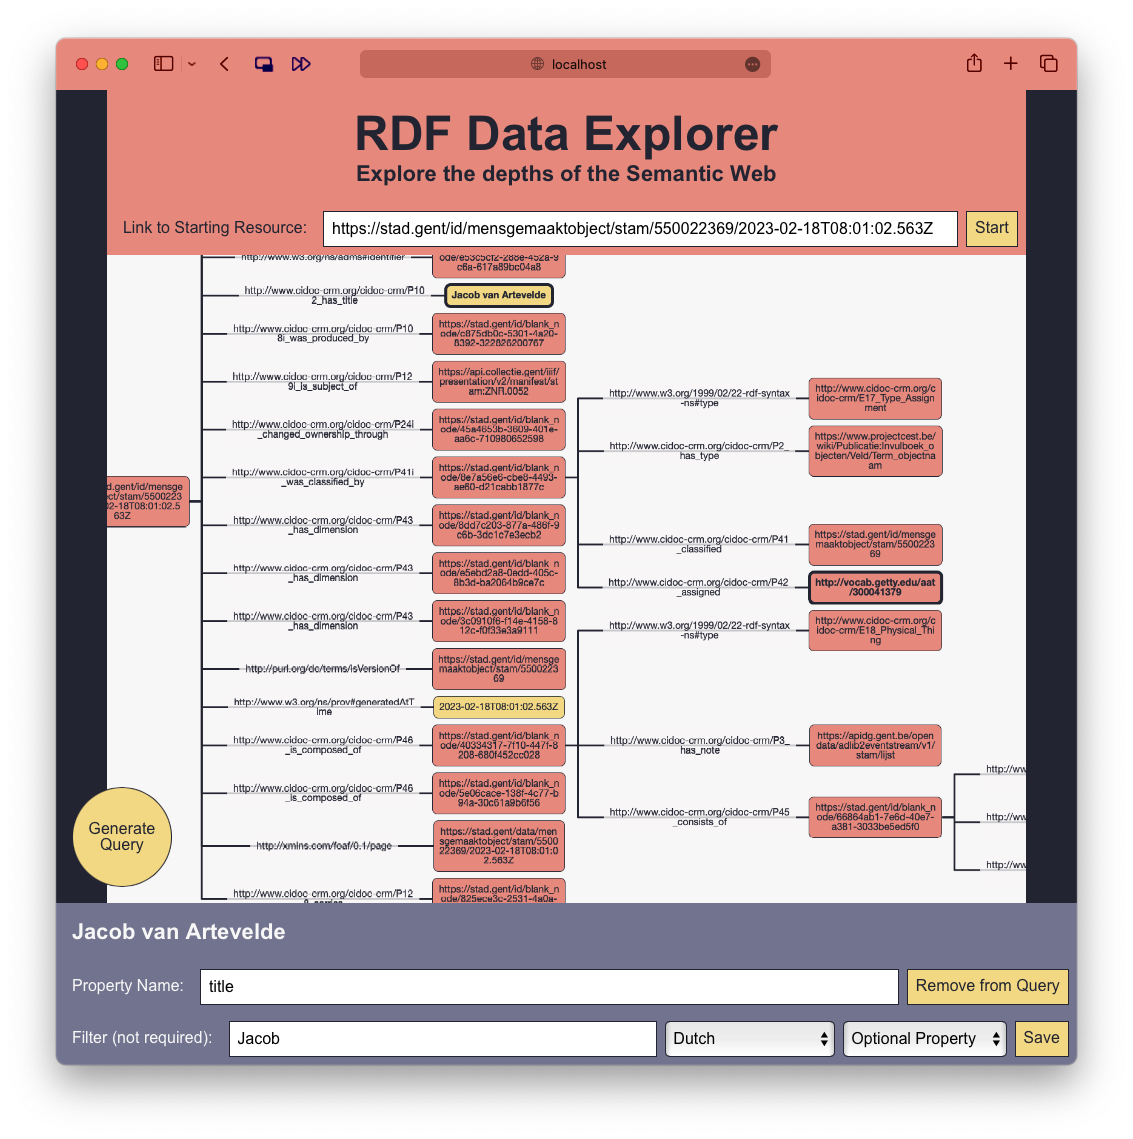
\includegraphics[width=\textwidth]{images/rdf_explorer.png}
	\caption{Screenshot of RDF Predicates Explorer}
	\label{fig:rdf_explorer}
\end{figure}

\subsection{Tree Expansion}

Another advantage to using \textit{cytoscape.js} is the ease with which event listeners for node clicks can be added. This is necessary as users need to interact with nodes. For instance, if a node represents a resource, not an atomic value, users should be able to \textit{expand} it. This involves retrieving the predicate and object for every triple pattern in which the resource is the subject. Consequently, for each such predicate-object pair found, a corresponding edge-node pair is added to the resource node. This system allows users to build a tree of predicates and resources, providing insights into the part of the web of Linked Data that the starting resource grants access to.

Naturally, behind this \textit{expanding} operation lies a SPARQL query. That query is not at all complicated, as exemplified by Code Fragment~\ref{lst:function_query_subject}. Here, the function that returns the necessary query for a given resource URI is presented. To execute the query, the application uses Comunica's standard SPARQL engine\footnote{\url{https://github.com/comunica/comunica/tree/master/engines/query-sparql}}, rather than a link traversal engine. The latter isn't necessary for this type of query, as there is no need for a link traversal engine that might needlessly search for potentially \textit{followable} links and carries some overhead anyways. Furthermore, the used query engine naturally requires a datasource. Logically, the resource URI should suffice for this. At least, that is the theory. Because in practice and as attested to in Section~\ref{sec:links_to_follow}, certain resource URIs – for various reasons – do not always lead directly to a \textit{queryable} document. For instance, Getty Vocabularies URIs only return correct JSON-LD content when a \mintinline{text}{.json-ld} extension is appended to them. Therefore, to also enable users to expand these \textit{affected} resources, the application provides the possibility to modify the datasource before executing the query from Code Fragment~\ref{lst:function_query_subject}. As a bonus, this also enables users to specify a SPARQL endpoint as the datasource, potentially speeding up querying.

\begin{listing}[htbp]
    \begin{minted}[samepage,fontsize=\small]{javascript}
function buildQuery(subjectResource) {
    return `
        SELECT ?p ?o
        WHERE {
            <${subjectResource}> ?p ?o.
        }
    `;
}
    \end{minted}
    \caption{Function returning a SPARQL query for completing a resource subject's triple pattern}
    \label{lst:function_query_subject}
\end{listing}

\subsection{Predicate Sequences Selection}

The purpose of the application central to this section is, of course, to compose queries. To achieve this, this application also utilizes the query builder application discussed in Section~\ref{sec:building_queries_predicate_sequences}. The query builder function of the latter expects several parameters, with the most important being the \mintinline{text}{properties} parameter. In other words, for each type of property the user wants to include in their query, at least the corresponding \textit{predicate sequence}, and optionally some filter details and an \mintinline{text}{optional} value, must be provided. Compiling all of this into a valid \mintinline{text}{properties} dictionary is a trivial task for the application. However, to understand the user's preferences, the necessary UI elements need to be provided. Code Fragment~\ref{fig:rdf_explorer} already provides a visual indication of those.

Specifically, the application presents an input form when a node is clicked. Initially, it only offers the option to enter a property name. The intention is for this to briefly describe the type of data obtained by following the predicate sequence to the node in question – whether a resource or an atomic value. Subsequently, once the property name is provided, the user can add the property to the query. This step presents them with a few additional yet optional fields. Specifically, the user can provide a string filter – the label of the node in question is automatically offered as an option – choose a language, and designate the property as required or optional. Each node included as a property in the query is highlighted in the tree.

Consequently, when the user is satisfied with their choices, they can press the \textit{Generate Query} button. Upon this signal, the application first collects all properties with their respective details into a dictionary, structured according to the rules defined in Section~\ref{subsec:building_queries_predicate_sequences_overview}. For each chosen node, this also requires the various predicates leading from the starting resource to that node. Fortunately, \textit{cytoscape.js} can help with this too. After all, for each node, it offers the \mintinline{text}{predecessors()}\footnote{\url{https://js.cytoscape.org/\#nodes.predecessors}} function. This leaves the application only with filtering each selected node's predecessors for just edges – predicates – and reversing their order. Eventually, once the complete \mintinline{text}{predicates} dictionary is determined, the application passes it to the query-building function, which ultimately presents the generated query to the user. As an added bonus, the application can even convert the dictionary to a JSON file, allowing it to be used as a \textit{module} in the application discussed in Section~\ref{sec:new_query_builder}.

\section{Conclusion}

The applications presented in Sections~\ref{sec:new_query_builder} and~\ref{sec:discovering_predicate_sequences} are primarily user-centric. The application in Section~\ref{sec:new_query_builder}, for instance, serves as a great starting point for absolute beginners to get a high-level idea of certain datasets, as well as how the selection of specific properties, accompanied by questions, translates into the construction of a SPARQL query. However, the drawback is that users rely on existing \textit{modules} tailored to specific datasets. Without these modules, the application has no use. This is why the application discussed in Section~\ref{sec:discovering_predicate_sequences} was developed. It allows users to select properties based on the branches and sub-branches of a specific resource in their dataset. However, this application expects a bit more technical understanding from users. Not only do users need to provide the URI of the starting resource themselves, \textit{expanding} the tree can also be a somewhat tedious process.

Certainly, both applications have their distinct strengths and weaknesses. However, the key functionality of both, which is query building, is performed by a separate application. This application provides a query-building function that enables developers to build various user-centric applications \textit{around} it. The only prerequisite is to provide the function with the appropriate parameters. Once again, the specific details of these parameters are set out in Section~\ref{subsec:building_queries_predicate_sequences_overview}.
\chapter{Handling Query Results}
\label{chap:handling_query_results}

TODO

\section{Visualizing Query Results}
\label{sec:visualizing_query_results}

TODO

\subsection{IIIF Viewers}

TODO

\subsection{Custom Viewer}

TODO

\section{Saving Query Results}
\label{sec:saving_query_results}

TODO

\subsection{SPARQL Query}

TODO

\subsection{IIIF Manifest}

TODO

\subsection{Predicate Sequences}

TODO

\section{Conclusion}

TODO
\chapter*{Conclusion}
\chaptermark{Conclusion}
\addcontentsline{toc}{chapter}{Conclusion}

The exploration of digital art collections using Link-Traversal–based Query Processing has been a multifaceted journey, intertwining the realms of art and technology. As digital art collections have become more accessible, challenges have arisen, particularly for individuals without a technical background. This research embarked on addressing these challenges, aiming to provide tools and methodologies that empower both professionals and art enthusiasts to delve deeper into the digital art landscape, making new discoveries and drawing meaningful connections.

The systematic process of discovering digital art collections can be broadly categorized into three main steps: building queries, executing them — with a specific focus on link traversal in this research — and handling the results through visualization and storage. Each chapter of this research has meticulously addressed one of these steps.

Chapter~\ref{chap:coghent_link_traversal} delved into the execution of queries using Link-Traversal-based Query Processing. The chapter emphasized the potential of link traversal in uncovering specific attributes of the Collections of Ghent's Human-Made Objects, offering insights that would remain hidden with traditional querying methods. However, it also highlighted the inherent challenges and unpredictability associated with link traversal. For instance, due to server misconfigurations, certain resources like Stad Gent's could not be accessed, while the use of others', like Getty Vocabularies', required workarounds. These challenges underscored the fragility of Link Traversal-based Query Processing compared to traditional SPARQL querying.

Chapter~\ref{chap:tools_query_building} introduced tools that simplify the intricate task of query formulation, making it more accessible to a broader audience. While these tools are valuable, they are not presented as the definitive solutions. Instead, their core query-building functionality is designed to be modular, allowing others to adapt and use it for their own discovery applications.

Chapter~\ref{chap:handling_query_results} addressed the post-query phase, focusing on the visualization and preservation of query results. The chapter weighed the advantages and disadvantages of different visualization and preservation methods. However, it also highlighted areas for further exploration, such as the adaptability of visualization tools to real-time query updates and the potential for presenting query results as immersive, interactive narratives. These areas present exciting avenues for future research.

In conclusion, this research has provided valuable insights and tools for the discovery process of digital art collections, while also shedding light on the inherent challenges of the process. Specifically, the fragility of link traversal, its slower performance compared to traditional SPARQL querying, and the unpredictability of outcomes due to server misconfigurations or other unforeseen technical issues, pose significant hurdles. However, the undeniable potential of link traversal to uncover hidden data and offer deeper insights into digital art collections offers a promising future. As technology evolves and these challenges are addressed, it is anticipated that link traversal and its associated tools will become more mainstream, benefiting a wider audience. Yet, it is important to note that, at the time of this research's publication, harnessing its full capabilities still demands a certain level of technical expertise.

\phantomsection
\section*{Ethical and social reflection}
\addcontentsline{toc}{section}{Ethical and social reflection}

In examining the ethical and societal dimensions of the research, it is instructive to consider its alignment with the 17 \textit{Sustainable Development Goals}\footnote{\url{https://sdgs.un.org/goals}} (SDG) of the United Nations' \textit{2030 Agenda for Sustainable Development}\footnote{\url{https://sdgs.un.org/2030agenda}}.

Primarily, the research's emphasis on open-source applications seeks to broaden access to the discovery of art and culture, irrespective of technical expertise. This approach has parallels with \textbf{SDG 4}\footnote{\url{https://sdgs.un.org/goals/goal4}}, which highlights inclusive education, and \textbf{SDG 10}\footnote{\url{https://sdgs.un.org/goals/goal10}}, which addresses the reduction of inequalities.

Furthermore, the use of Linked Open Data in the research provides a mechanism for global cultural representation. With the study primarily focusing on Ghent's cultural heritage, its objectives intersect with \textbf{SDG 11}\footnote{\url{https://sdgs.un.org/goals/goal11}}, which is concerned with the preservation of global cultural heritage. The collaborative nature of the CoGhent partnership also reflects the spirit of \textbf{SDG 17}\footnote{\url{https://sdgs.un.org/goals/goal17}}, which underscores the importance of partnerships.

The research's utilization of the semantic web offers a method for accessible art collection discovery, which can be related to \textbf{SDGs 8}\footnote{\url{https://sdgs.un.org/goals/goal8}} and \textbf{9}\footnote{\url{https://sdgs.un.org/goals/goal9}}, centered around economic growth and innovation. Additionally, the semantic web's approach to data control aligns with \textbf{SDG 16}'s\footnote{\url{https://sdgs.un.org/goals/goal16}} emphasis on transparency and accountability.

In summary, although the research does not \textit{directly} address \textit{all} the SDGs mentioned above, its utilization of the semantic web and the introduction of various open-source tools at least provide \textit{avenues} for potentially aligning with them.
\renewcommand\bibname{References}
\bibliography{references}

\pagestyle{numberless} 
\pagestyle{empty}
\begin{appendices}
\section*{Appendix A}
\addcontentsline{toc}{section}{Appendix A}  

TODO

\newpage
\section*{Appendix B}
\addcontentsline{toc}{section}{Appendix B}  

TODO

\end{appendices}


\end{document}
